\begin{tikzpicture}[scale=.2, anchor=south west]
\node[draw=black, rectangle split, rectangle split parts=3] (sn0x920fc60W-5) at (-5.5, -12) {
\begin{tikzpicture}[scale=.2]
\node[circle, scale=0.75, fill] (tid0) at (4.5,0){};
\node[circle, scale=0.75, fill] (tid1) at (2.25,1.5){};
\node[circle, scale=0.75, fill, red] (tid4) at (0.75,3){};
\node[circle, scale=0.75, fill, red] (tid5) at (2.25,3){};
\node[circle, scale=0.75, fill] (tid6) at (3.75,3){};
\draw[](tid1) -- (tid4);
\draw[](tid1) -- (tid5);
\draw[](tid1) -- (tid6);
\node[circle, scale=0.75, fill] (tid2) at (6,1.5){};
\node[circle, scale=0.75, fill, red] (tid7) at (5.25,3){};
\node[circle, scale=0.75, fill] (tid8) at (6.75,3){};
\draw[](tid2) -- (tid7);
\draw[](tid2) -- (tid8);
\node[circle, scale=0.75, fill] (tid3) at (8.25,1.5){};
\node[circle, scale=0.75, fill] (tid9) at (8.25,3){};
\draw[](tid3) -- (tid9);
\draw[](tid0) -- (tid1);
\draw[](tid0) -- (tid2);
\draw[](tid0) -- (tid3);

\end{tikzpicture}
\nodepart{two}
\footnotesize{5.20782}
\nodepart{three}
\footnotesize{0.22 0.22 0.22 0.11 0.11 0.11}
};
\node[draw=black, rectangle split, rectangle split parts=3] (sn0x920e170W-28) at (-28.5, -24) {
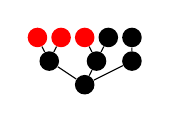
\begin{tikzpicture}[scale=.2]
\node[circle, scale=0.75, fill] (tid0) at (3.75,0){};
\node[circle, scale=0.75, fill] (tid1) at (1.5,1.5){};
\node[circle, scale=0.75, fill, red] (tid4) at (0.75,3){};
\node[circle, scale=0.75, fill, red] (tid5) at (2.25,3){};
\draw[](tid1) -- (tid4);
\draw[](tid1) -- (tid5);
\node[circle, scale=0.75, fill] (tid2) at (4.5,1.5){};
\node[circle, scale=0.75, fill, red] (tid6) at (3.75,3){};
\node[circle, scale=0.75, fill] (tid7) at (5.25,3){};
\draw[](tid2) -- (tid6);
\draw[](tid2) -- (tid7);
\node[circle, scale=0.75, fill] (tid3) at (6.75,1.5){};
\node[circle, scale=0.75, fill] (tid8) at (6.75,3){};
\draw[](tid3) -- (tid8);
\draw[](tid0) -- (tid1);
\draw[](tid0) -- (tid2);
\draw[](tid0) -- (tid3);

\end{tikzpicture}
\nodepart{two}
\footnotesize{4.87551}
\nodepart{three}
\footnotesize{0.5 0.33 0.17}
};
\node[draw=black, rectangle split, rectangle split parts=3] (sn0x9211948W-31) at (-31, -36) {
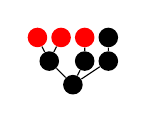
\begin{tikzpicture}[scale=.2]
\node[circle, scale=0.75, fill] (tid0) at (3,0){};
\node[circle, scale=0.75, fill] (tid1) at (1.5,1.5){};
\node[circle, scale=0.75, fill, red] (tid4) at (0.75,3){};
\node[circle, scale=0.75, fill, red] (tid5) at (2.25,3){};
\draw[](tid1) -- (tid4);
\draw[](tid1) -- (tid5);
\node[circle, scale=0.75, fill] (tid2) at (3.75,1.5){};
\node[circle, scale=0.75, fill, red] (tid6) at (3.75,3){};
\draw[](tid2) -- (tid6);
\node[circle, scale=0.75, fill] (tid3) at (5.25,1.5){};
\node[circle, scale=0.75, fill] (tid7) at (5.25,3){};
\draw[](tid3) -- (tid7);
\draw[](tid0) -- (tid1);
\draw[](tid0) -- (tid2);
\draw[](tid0) -- (tid3);

\end{tikzpicture}
\nodepart{two}
\footnotesize{4.54321}
\nodepart{three}
\footnotesize{0.67 0.33}
};
\node[draw=black, rectangle split, rectangle split parts=3] (sn0x920f510W-12) at (-12, -48) {
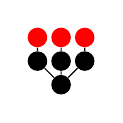
\begin{tikzpicture}[scale=.2]
\node[circle, scale=0.75, fill] (tid0) at (2.25,0){};
\node[circle, scale=0.75, fill] (tid1) at (0.75,1.5){};
\node[circle, scale=0.75, fill, red] (tid4) at (0.75,3){};
\draw[](tid1) -- (tid4);
\node[circle, scale=0.75, fill] (tid2) at (2.25,1.5){};
\node[circle, scale=0.75, fill, red] (tid5) at (2.25,3){};
\draw[](tid2) -- (tid5);
\node[circle, scale=0.75, fill] (tid3) at (3.75,1.5){};
\node[circle, scale=0.75, fill, red] (tid6) at (3.75,3){};
\draw[](tid3) -- (tid6);
\draw[](tid0) -- (tid1);
\draw[](tid0) -- (tid2);
\draw[](tid0) -- (tid3);

\end{tikzpicture}
\nodepart{two}
\footnotesize{4.21296}
\nodepart{three}
\footnotesize{1}
};
\node[draw=black, rectangle split, rectangle split parts=3] (sn0x9210968W-7) at (-7.25, -60) {
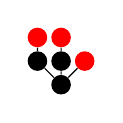
\begin{tikzpicture}[scale=.2]
\node[circle, scale=0.75, fill] (tid0) at (2.25,0){};
\node[circle, scale=0.75, fill] (tid1) at (0.75,1.5){};
\node[circle, scale=0.75, fill, red] (tid4) at (0.75,3){};
\draw[](tid1) -- (tid4);
\node[circle, scale=0.75, fill] (tid2) at (2.25,1.5){};
\node[circle, scale=0.75, fill, red] (tid5) at (2.25,3){};
\draw[](tid2) -- (tid5);
\node[circle, scale=0.75, fill, red] (tid3) at (3.75,1.5){};
\draw[](tid0) -- (tid1);
\draw[](tid0) -- (tid2);
\draw[](tid0) -- (tid3);

\end{tikzpicture}
\nodepart{two}
\footnotesize{3.87963}
\nodepart{three}
\footnotesize{0.33 0.67}
};
\node[draw=black, rectangle split, rectangle split parts=3] (sn0x9210b90W-9) at (-9, -72) {
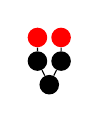
\begin{tikzpicture}[scale=.2]
\node[circle, scale=0.75, fill] (tid0) at (1.5,0){};
\node[circle, scale=0.75, fill] (tid1) at (0.75,1.5){};
\node[circle, scale=0.75, fill, red] (tid3) at (0.75,3){};
\draw[](tid1) -- (tid3);
\node[circle, scale=0.75, fill] (tid2) at (2.25,1.5){};
\node[circle, scale=0.75, fill, red] (tid4) at (2.25,3){};
\draw[](tid2) -- (tid4);
\draw[](tid0) -- (tid1);
\draw[](tid0) -- (tid2);

\end{tikzpicture}
\nodepart{two}
\footnotesize{3.75}
\nodepart{three}
\footnotesize{1}
};
\node[draw=black, rectangle split, rectangle split parts=3] (sn0x9210d88W-8) at (-8.25, -84) {
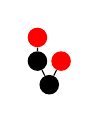
\begin{tikzpicture}[scale=.2]
\node[circle, scale=0.75, fill] (tid0) at (1.5,0){};
\node[circle, scale=0.75, fill] (tid1) at (0.75,1.5){};
\node[circle, scale=0.75, fill, red] (tid3) at (0.75,3){};
\draw[](tid1) -- (tid3);
\node[circle, scale=0.75, fill, red] (tid2) at (2.25,1.5){};
\draw[](tid0) -- (tid1);
\draw[](tid0) -- (tid2);

\end{tikzpicture}
\nodepart{two}
\footnotesize{3.25}
\nodepart{three}
\footnotesize{0.5 0.5}
};
\node[draw=black, rectangle split, rectangle split parts=3] (sn0x9210f38W-4) at (-4.25, -96) {
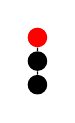
\begin{tikzpicture}[scale=.2]
\node[circle, scale=0.75, fill] (tid0) at (0.75,0){};
\node[circle, scale=0.75, fill] (tid1) at (0.75,1.5){};
\node[circle, scale=0.75, fill, red] (tid2) at (0.75,3){};
\draw[](tid1) -- (tid2);
\draw[](tid0) -- (tid1);

\end{tikzpicture}
\nodepart{two}
\footnotesize{3}
\nodepart{three}
\footnotesize{1}
};
\node[draw=black, rectangle split, rectangle split parts=3] (sn0x9211160W-1) at (-1.75, -108) {

\begin{tikzpicture}[scale=.2]
\node[circle, scale=0.75, fill] (tid0) at (0.75,0){};
\node[circle, scale=0.75, fill, red] (tid1) at (0.75,1.5){};
\draw[](tid0) -- (tid1);

\end{tikzpicture}
\nodepart{two}
\footnotesize{2}
\nodepart{three}
\footnotesize{1}
};
\node[draw=black, rectangle split, rectangle split parts=3] (sn0x92111d8W-1) at (-1.75, -120) {

\begin{tikzpicture}[scale=.2]
\node[circle, scale=0.75, fill, red] (tid0) at (0.75,0){};

\end{tikzpicture}
\nodepart{two}
\footnotesize{1}
\nodepart{three}
\footnotesize{}
};
\draw (sn0x9211160W-1.south) -- (sn0x92111d8W-1.north);
\draw (sn0x9210f38W-4.south) -- (sn0x9211160W-1.north);
\node[draw=black, rectangle split, rectangle split parts=3] (sn0x9210fa0W0) at (-0.75, -96) {

\begin{tikzpicture}[scale=.2]
\node[circle, scale=0.75, fill] (tid0) at (1.5,0){};
\node[circle, scale=0.75, fill, red] (tid1) at (0.75,1.5){};
\node[circle, scale=0.75, fill, red] (tid2) at (2.25,1.5){};
\draw[](tid0) -- (tid1);
\draw[](tid0) -- (tid2);

\end{tikzpicture}
\nodepart{two}
\footnotesize{2.5}
\nodepart{three}
\footnotesize{1}
};
\draw (sn0x9210fa0W0.south) -- (sn0x9211160W-1.north);
\draw (sn0x9210d88W-8.south) -- (sn0x9210f38W-4.north);
\draw (sn0x9210d88W-8.south) -- (sn0x9210fa0W0.north);
\draw (sn0x9210b90W-9.south) -- (sn0x9210d88W-8.north);
\node[draw=black, rectangle split, rectangle split parts=3] (sn0x9210c28W-4) at (-4, -72) {
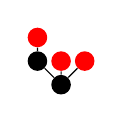
\begin{tikzpicture}[scale=.2]
\node[circle, scale=0.75, fill] (tid0) at (2.25,0){};
\node[circle, scale=0.75, fill] (tid1) at (0.75,1.5){};
\node[circle, scale=0.75, fill, red] (tid4) at (0.75,3){};
\draw[](tid1) -- (tid4);
\node[circle, scale=0.75, fill, red] (tid2) at (2.25,1.5){};
\node[circle, scale=0.75, fill, red] (tid3) at (3.75,1.5){};
\draw[](tid0) -- (tid1);
\draw[](tid0) -- (tid2);
\draw[](tid0) -- (tid3);

\end{tikzpicture}
\nodepart{two}
\footnotesize{3.44444}
\nodepart{three}
\footnotesize{0.67 0.33}
};
\node[draw=black, rectangle split, rectangle split parts=3] (sn0x9215aa8W-3) at (-3.25, -84) {
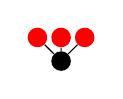
\begin{tikzpicture}[scale=.2]
\node[circle, scale=0.75, fill] (tid0) at (2.25,0){};
\node[circle, scale=0.75, fill, red] (tid1) at (0.75,1.5){};
\node[circle, scale=0.75, fill, red] (tid2) at (2.25,1.5){};
\node[circle, scale=0.75, fill, red] (tid3) at (3.75,1.5){};
\draw[](tid0) -- (tid1);
\draw[](tid0) -- (tid2);
\draw[](tid0) -- (tid3);

\end{tikzpicture}
\nodepart{two}
\footnotesize{2.83333}
\nodepart{three}
\footnotesize{1}
};
\draw (sn0x9215aa8W-3.south) -- (sn0x9210fa0W0.north);
\draw (sn0x9210c28W-4.south) -- (sn0x9210d88W-8.north);
\draw (sn0x9210c28W-4.south) -- (sn0x9215aa8W-3.north);
\draw (sn0x9210968W-7.south) -- (sn0x9210b90W-9.north);
\draw (sn0x9210968W-7.south) -- (sn0x9210c28W-4.north);
\draw (sn0x920f510W-12.south) -- (sn0x9210968W-7.north);
\node[draw=black, rectangle split, rectangle split parts=3] (sn0x92105f0W-5) at (-5.5, -48) {
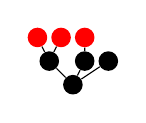
\begin{tikzpicture}[scale=.2]
\node[circle, scale=0.75, fill] (tid0) at (3,0){};
\node[circle, scale=0.75, fill] (tid1) at (1.5,1.5){};
\node[circle, scale=0.75, fill, red] (tid4) at (0.75,3){};
\node[circle, scale=0.75, fill, red] (tid5) at (2.25,3){};
\draw[](tid1) -- (tid4);
\draw[](tid1) -- (tid5);
\node[circle, scale=0.75, fill] (tid2) at (3.75,1.5){};
\node[circle, scale=0.75, fill, red] (tid6) at (3.75,3){};
\draw[](tid2) -- (tid6);
\node[circle, scale=0.75, fill] (tid3) at (5.25,1.5){};
\draw[](tid0) -- (tid1);
\draw[](tid0) -- (tid2);
\draw[](tid0) -- (tid3);

\end{tikzpicture}
\nodepart{two}
\footnotesize{4.2037}
\nodepart{three}
\footnotesize{0.67 0.33}
};
\node[draw=black, rectangle split, rectangle split parts=3] (sn0x9215e90W0) at (-0.75, -60) {
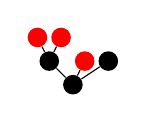
\begin{tikzpicture}[scale=.2]
\node[circle, scale=0.75, fill] (tid0) at (3,0){};
\node[circle, scale=0.75, fill] (tid1) at (1.5,1.5){};
\node[circle, scale=0.75, fill, red] (tid4) at (0.75,3){};
\node[circle, scale=0.75, fill, red] (tid5) at (2.25,3){};
\draw[](tid1) -- (tid4);
\draw[](tid1) -- (tid5);
\node[circle, scale=0.75, fill, red] (tid2) at (3.75,1.5){};
\node[circle, scale=0.75, fill] (tid3) at (5.25,1.5){};
\draw[](tid0) -- (tid1);
\draw[](tid0) -- (tid2);
\draw[](tid0) -- (tid3);

\end{tikzpicture}
\nodepart{two}
\footnotesize{3.85185}
\nodepart{three}
\footnotesize{0.33 0.67}
};
\node[draw=black, rectangle split, rectangle split parts=3] (sn0x9216188W2) at (2.5, -72) {
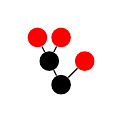
\begin{tikzpicture}[scale=.2]
\node[circle, scale=0.75, fill] (tid0) at (2.25,0){};
\node[circle, scale=0.75, fill] (tid1) at (1.5,1.5){};
\node[circle, scale=0.75, fill, red] (tid3) at (0.75,3){};
\node[circle, scale=0.75, fill, red] (tid4) at (2.25,3){};
\draw[](tid1) -- (tid3);
\draw[](tid1) -- (tid4);
\node[circle, scale=0.75, fill, red] (tid2) at (3.75,1.5){};
\draw[](tid0) -- (tid1);
\draw[](tid0) -- (tid2);

\end{tikzpicture}
\nodepart{two}
\footnotesize{3.66667}
\nodepart{three}
\footnotesize{0.33 0.67}
};
\node[draw=black, rectangle split, rectangle split parts=3] (sn0x9215c40W3) at (3.25, -84) {
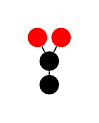
\begin{tikzpicture}[scale=.2]
\node[circle, scale=0.75, fill] (tid0) at (1.5,0){};
\node[circle, scale=0.75, fill] (tid1) at (1.5,1.5){};
\node[circle, scale=0.75, fill, red] (tid2) at (0.75,3){};
\node[circle, scale=0.75, fill, red] (tid3) at (2.25,3){};
\draw[](tid1) -- (tid2);
\draw[](tid1) -- (tid3);
\draw[](tid0) -- (tid1);

\end{tikzpicture}
\nodepart{two}
\footnotesize{3.5}
\nodepart{three}
\footnotesize{1}
};
\draw (sn0x9215c40W3.south) -- (sn0x9210f38W-4.north);
\draw (sn0x9216188W2.south) -- (sn0x9215c40W3.north);
\draw (sn0x9216188W2.south) -- (sn0x9210d88W-8.north);
\draw (sn0x9215e90W0.south) -- (sn0x9216188W2.north);
\draw (sn0x9215e90W0.south) -- (sn0x9210c28W-4.north);
\draw (sn0x92105f0W-5.south) -- (sn0x9210968W-7.north);
\draw (sn0x92105f0W-5.south) -- (sn0x9215e90W0.north);
\draw (sn0x9211948W-31.south) -- (sn0x920f510W-12.north);
\draw (sn0x9211948W-31.south) -- (sn0x92105f0W-5.north);
\node[draw=black, rectangle split, rectangle split parts=3] (sn0x92115d8W-23) at (-23, -36) {
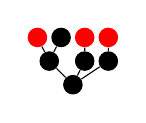
\begin{tikzpicture}[scale=.2]
\node[circle, scale=0.75, fill] (tid0) at (3,0){};
\node[circle, scale=0.75, fill] (tid1) at (1.5,1.5){};
\node[circle, scale=0.75, fill, red] (tid4) at (0.75,3){};
\node[circle, scale=0.75, fill] (tid5) at (2.25,3){};
\draw[](tid1) -- (tid4);
\draw[](tid1) -- (tid5);
\node[circle, scale=0.75, fill] (tid2) at (3.75,1.5){};
\node[circle, scale=0.75, fill, red] (tid6) at (3.75,3){};
\draw[](tid2) -- (tid6);
\node[circle, scale=0.75, fill] (tid3) at (5.25,1.5){};
\node[circle, scale=0.75, fill, red] (tid7) at (5.25,3){};
\draw[](tid3) -- (tid7);
\draw[](tid0) -- (tid1);
\draw[](tid0) -- (tid2);
\draw[](tid0) -- (tid3);

\end{tikzpicture}
\nodepart{two}
\footnotesize{4.54012}
\nodepart{three}
\footnotesize{0.33 0.67}
};
\draw (sn0x92115d8W-23.south) -- (sn0x920f510W-12.north);
\draw (sn0x92115d8W-23.south) -- (sn0x92105f0W-5.north);
\node[draw=black, rectangle split, rectangle split parts=3] (sn0x920f478W-15) at (-15, -36) {
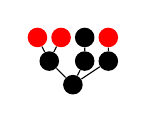
\begin{tikzpicture}[scale=.2]
\node[circle, scale=0.75, fill] (tid0) at (3,0){};
\node[circle, scale=0.75, fill] (tid1) at (1.5,1.5){};
\node[circle, scale=0.75, fill, red] (tid4) at (0.75,3){};
\node[circle, scale=0.75, fill, red] (tid5) at (2.25,3){};
\draw[](tid1) -- (tid4);
\draw[](tid1) -- (tid5);
\node[circle, scale=0.75, fill] (tid2) at (3.75,1.5){};
\node[circle, scale=0.75, fill] (tid6) at (3.75,3){};
\draw[](tid2) -- (tid6);
\node[circle, scale=0.75, fill] (tid3) at (5.25,1.5){};
\node[circle, scale=0.75, fill, red] (tid7) at (5.25,3){};
\draw[](tid3) -- (tid7);
\draw[](tid0) -- (tid1);
\draw[](tid0) -- (tid2);
\draw[](tid0) -- (tid3);

\end{tikzpicture}
\nodepart{two}
\footnotesize{4.54321}
\nodepart{three}
\footnotesize{0.67 0.33}
};
\draw (sn0x920f478W-15.south) -- (sn0x920f510W-12.north);
\draw (sn0x920f478W-15.south) -- (sn0x92105f0W-5.north);
\draw (sn0x920e170W-28.south) -- (sn0x9211948W-31.north);
\draw (sn0x920e170W-28.south) -- (sn0x92115d8W-23.north);
\draw (sn0x920e170W-28.south) -- (sn0x920f478W-15.north);
\node[draw=black, rectangle split, rectangle split parts=3] (sn0x92150f0W-19) at (-19, -24) {
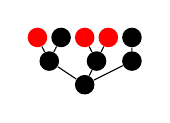
\begin{tikzpicture}[scale=.2]
\node[circle, scale=0.75, fill] (tid0) at (3.75,0){};
\node[circle, scale=0.75, fill] (tid1) at (1.5,1.5){};
\node[circle, scale=0.75, fill, red] (tid4) at (0.75,3){};
\node[circle, scale=0.75, fill] (tid5) at (2.25,3){};
\draw[](tid1) -- (tid4);
\draw[](tid1) -- (tid5);
\node[circle, scale=0.75, fill] (tid2) at (4.5,1.5){};
\node[circle, scale=0.75, fill, red] (tid6) at (3.75,3){};
\node[circle, scale=0.75, fill, red] (tid7) at (5.25,3){};
\draw[](tid2) -- (tid6);
\draw[](tid2) -- (tid7);
\node[circle, scale=0.75, fill] (tid3) at (6.75,1.5){};
\node[circle, scale=0.75, fill] (tid8) at (6.75,3){};
\draw[](tid3) -- (tid8);
\draw[](tid0) -- (tid1);
\draw[](tid0) -- (tid2);
\draw[](tid0) -- (tid3);

\end{tikzpicture}
\nodepart{two}
\footnotesize{4.87551}
\nodepart{three}
\footnotesize{0.5 0.17 0.33}
};
\draw (sn0x92150f0W-19.south) -- (sn0x9211948W-31.north);
\draw (sn0x92150f0W-19.south) -- (sn0x920f478W-15.north);
\draw (sn0x92150f0W-19.south) -- (sn0x92115d8W-23.north);
\node[draw=black, rectangle split, rectangle split parts=3] (sn0x920f210W-9) at (-9.5, -24) {
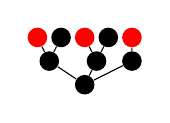
\begin{tikzpicture}[scale=.2]
\node[circle, scale=0.75, fill] (tid0) at (3.75,0){};
\node[circle, scale=0.75, fill] (tid1) at (1.5,1.5){};
\node[circle, scale=0.75, fill, red] (tid4) at (0.75,3){};
\node[circle, scale=0.75, fill] (tid5) at (2.25,3){};
\draw[](tid1) -- (tid4);
\draw[](tid1) -- (tid5);
\node[circle, scale=0.75, fill] (tid2) at (4.5,1.5){};
\node[circle, scale=0.75, fill, red] (tid6) at (3.75,3){};
\node[circle, scale=0.75, fill] (tid7) at (5.25,3){};
\draw[](tid2) -- (tid6);
\draw[](tid2) -- (tid7);
\node[circle, scale=0.75, fill] (tid3) at (6.75,1.5){};
\node[circle, scale=0.75, fill, red] (tid8) at (6.75,3){};
\draw[](tid3) -- (tid8);
\draw[](tid0) -- (tid1);
\draw[](tid0) -- (tid2);
\draw[](tid0) -- (tid3);

\end{tikzpicture}
\nodepart{two}
\footnotesize{4.87346}
\nodepart{three}
\footnotesize{0.33 0.33 0.17 0.17}
};
\node[draw=black, rectangle split, rectangle split parts=3] (sn0x9215cf0W-7) at (-7, -36) {
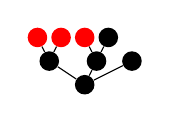
\begin{tikzpicture}[scale=.2]
\node[circle, scale=0.75, fill] (tid0) at (3.75,0){};
\node[circle, scale=0.75, fill] (tid1) at (1.5,1.5){};
\node[circle, scale=0.75, fill, red] (tid4) at (0.75,3){};
\node[circle, scale=0.75, fill, red] (tid5) at (2.25,3){};
\draw[](tid1) -- (tid4);
\draw[](tid1) -- (tid5);
\node[circle, scale=0.75, fill] (tid2) at (4.5,1.5){};
\node[circle, scale=0.75, fill, red] (tid6) at (3.75,3){};
\node[circle, scale=0.75, fill] (tid7) at (5.25,3){};
\draw[](tid2) -- (tid6);
\draw[](tid2) -- (tid7);
\node[circle, scale=0.75, fill] (tid3) at (6.75,1.5){};
\draw[](tid0) -- (tid1);
\draw[](tid0) -- (tid2);
\draw[](tid0) -- (tid3);

\end{tikzpicture}
\nodepart{two}
\footnotesize{4.53704}
\nodepart{three}
\footnotesize{1}
};
\draw (sn0x9215cf0W-7.south) -- (sn0x92105f0W-5.north);
\node[draw=black, rectangle split, rectangle split parts=3] (sn0x9216a40W2) at (2.5, -36) {
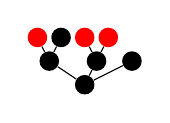
\begin{tikzpicture}[scale=.2]
\node[circle, scale=0.75, fill] (tid0) at (3.75,0){};
\node[circle, scale=0.75, fill] (tid1) at (1.5,1.5){};
\node[circle, scale=0.75, fill, red] (tid4) at (0.75,3){};
\node[circle, scale=0.75, fill] (tid5) at (2.25,3){};
\draw[](tid1) -- (tid4);
\draw[](tid1) -- (tid5);
\node[circle, scale=0.75, fill] (tid2) at (4.5,1.5){};
\node[circle, scale=0.75, fill, red] (tid6) at (3.75,3){};
\node[circle, scale=0.75, fill, red] (tid7) at (5.25,3){};
\draw[](tid2) -- (tid6);
\draw[](tid2) -- (tid7);
\node[circle, scale=0.75, fill] (tid3) at (6.75,1.5){};
\draw[](tid0) -- (tid1);
\draw[](tid0) -- (tid2);
\draw[](tid0) -- (tid3);

\end{tikzpicture}
\nodepart{two}
\footnotesize{4.53704}
\nodepart{three}
\footnotesize{1}
};
\draw (sn0x9216a40W2.south) -- (sn0x92105f0W-5.north);
\draw (sn0x920f210W-9.south) -- (sn0x92115d8W-23.north);
\draw (sn0x920f210W-9.south) -- (sn0x920f478W-15.north);
\draw (sn0x920f210W-9.south) -- (sn0x9215cf0W-7.north);
\draw (sn0x920f210W-9.south) -- (sn0x9216a40W2.north);
\node[draw=black, rectangle split, rectangle split parts=3] (sn0x92141f0W0) at (0, -24) {
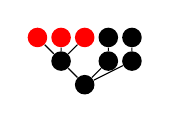
\begin{tikzpicture}[scale=.2]
\node[circle, scale=0.75, fill] (tid0) at (3.75,0){};
\node[circle, scale=0.75, fill] (tid1) at (2.25,1.5){};
\node[circle, scale=0.75, fill, red] (tid4) at (0.75,3){};
\node[circle, scale=0.75, fill, red] (tid5) at (2.25,3){};
\node[circle, scale=0.75, fill, red] (tid6) at (3.75,3){};
\draw[](tid1) -- (tid4);
\draw[](tid1) -- (tid5);
\draw[](tid1) -- (tid6);
\node[circle, scale=0.75, fill] (tid2) at (5.25,1.5){};
\node[circle, scale=0.75, fill] (tid7) at (5.25,3){};
\draw[](tid2) -- (tid7);
\node[circle, scale=0.75, fill] (tid3) at (6.75,1.5){};
\node[circle, scale=0.75, fill] (tid8) at (6.75,3){};
\draw[](tid3) -- (tid8);
\draw[](tid0) -- (tid1);
\draw[](tid0) -- (tid2);
\draw[](tid0) -- (tid3);

\end{tikzpicture}
\nodepart{two}
\footnotesize{4.87654}
\nodepart{three}
\footnotesize{0.5 0.5}
};
\draw (sn0x92141f0W0.south) -- (sn0x9211948W-31.north);
\draw (sn0x92141f0W0.south) -- (sn0x920f478W-15.north);
\node[draw=black, rectangle split, rectangle split parts=3] (sn0x92154e0W9) at (9.5, -24) {
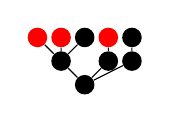
\begin{tikzpicture}[scale=.2]
\node[circle, scale=0.75, fill] (tid0) at (3.75,0){};
\node[circle, scale=0.75, fill] (tid1) at (2.25,1.5){};
\node[circle, scale=0.75, fill, red] (tid4) at (0.75,3){};
\node[circle, scale=0.75, fill, red] (tid5) at (2.25,3){};
\node[circle, scale=0.75, fill] (tid6) at (3.75,3){};
\draw[](tid1) -- (tid4);
\draw[](tid1) -- (tid5);
\draw[](tid1) -- (tid6);
\node[circle, scale=0.75, fill] (tid2) at (5.25,1.5){};
\node[circle, scale=0.75, fill, red] (tid7) at (5.25,3){};
\draw[](tid2) -- (tid7);
\node[circle, scale=0.75, fill] (tid3) at (6.75,1.5){};
\node[circle, scale=0.75, fill] (tid8) at (6.75,3){};
\draw[](tid3) -- (tid8);
\draw[](tid0) -- (tid1);
\draw[](tid0) -- (tid2);
\draw[](tid0) -- (tid3);

\end{tikzpicture}
\nodepart{two}
\footnotesize{4.87243}
\nodepart{three}
\footnotesize{0.33 0.33 0.17 0.17}
};
\node[draw=black, rectangle split, rectangle split parts=3] (sn0x9216c00W12) at (12, -36) {
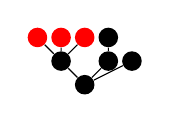
\begin{tikzpicture}[scale=.2]
\node[circle, scale=0.75, fill] (tid0) at (3.75,0){};
\node[circle, scale=0.75, fill] (tid1) at (2.25,1.5){};
\node[circle, scale=0.75, fill, red] (tid4) at (0.75,3){};
\node[circle, scale=0.75, fill, red] (tid5) at (2.25,3){};
\node[circle, scale=0.75, fill, red] (tid6) at (3.75,3){};
\draw[](tid1) -- (tid4);
\draw[](tid1) -- (tid5);
\draw[](tid1) -- (tid6);
\node[circle, scale=0.75, fill] (tid2) at (5.25,1.5){};
\node[circle, scale=0.75, fill] (tid7) at (5.25,3){};
\draw[](tid2) -- (tid7);
\node[circle, scale=0.75, fill] (tid3) at (6.75,1.5){};
\draw[](tid0) -- (tid1);
\draw[](tid0) -- (tid2);
\draw[](tid0) -- (tid3);

\end{tikzpicture}
\nodepart{two}
\footnotesize{4.53704}
\nodepart{three}
\footnotesize{1}
};
\draw (sn0x9216c00W12.south) -- (sn0x92105f0W-5.north);
\node[draw=black, rectangle split, rectangle split parts=3] (sn0x9217040W21) at (21.5, -36) {
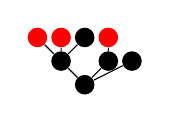
\begin{tikzpicture}[scale=.2]
\node[circle, scale=0.75, fill] (tid0) at (3.75,0){};
\node[circle, scale=0.75, fill] (tid1) at (2.25,1.5){};
\node[circle, scale=0.75, fill, red] (tid4) at (0.75,3){};
\node[circle, scale=0.75, fill, red] (tid5) at (2.25,3){};
\node[circle, scale=0.75, fill] (tid6) at (3.75,3){};
\draw[](tid1) -- (tid4);
\draw[](tid1) -- (tid5);
\draw[](tid1) -- (tid6);
\node[circle, scale=0.75, fill] (tid2) at (5.25,1.5){};
\node[circle, scale=0.75, fill, red] (tid7) at (5.25,3){};
\draw[](tid2) -- (tid7);
\node[circle, scale=0.75, fill] (tid3) at (6.75,1.5){};
\draw[](tid0) -- (tid1);
\draw[](tid0) -- (tid2);
\draw[](tid0) -- (tid3);

\end{tikzpicture}
\nodepart{two}
\footnotesize{4.53086}
\nodepart{three}
\footnotesize{0.67 0.33}
};
\node[draw=black, rectangle split, rectangle split parts=3] (sn0x9217148W2) at (2.5, -48) {
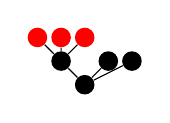
\begin{tikzpicture}[scale=.2]
\node[circle, scale=0.75, fill] (tid0) at (3.75,0){};
\node[circle, scale=0.75, fill] (tid1) at (2.25,1.5){};
\node[circle, scale=0.75, fill, red] (tid4) at (0.75,3){};
\node[circle, scale=0.75, fill, red] (tid5) at (2.25,3){};
\node[circle, scale=0.75, fill, red] (tid6) at (3.75,3){};
\draw[](tid1) -- (tid4);
\draw[](tid1) -- (tid5);
\draw[](tid1) -- (tid6);
\node[circle, scale=0.75, fill] (tid2) at (5.25,1.5){};
\node[circle, scale=0.75, fill] (tid3) at (6.75,1.5){};
\draw[](tid0) -- (tid1);
\draw[](tid0) -- (tid2);
\draw[](tid0) -- (tid3);

\end{tikzpicture}
\nodepart{two}
\footnotesize{4.18519}
\nodepart{three}
\footnotesize{1}
};
\draw (sn0x9217148W2.south) -- (sn0x9215e90W0.north);
\draw (sn0x9217040W21.south) -- (sn0x92105f0W-5.north);
\draw (sn0x9217040W21.south) -- (sn0x9217148W2.north);
\draw (sn0x92154e0W9.south) -- (sn0x9211948W-31.north);
\draw (sn0x92154e0W9.south) -- (sn0x92115d8W-23.north);
\draw (sn0x92154e0W9.south) -- (sn0x9216c00W12.north);
\draw (sn0x92154e0W9.south) -- (sn0x9217040W21.north);
\node[draw=black, rectangle split, rectangle split parts=3] (sn0x920ee08W19) at (19, -24) {
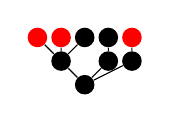
\begin{tikzpicture}[scale=.2]
\node[circle, scale=0.75, fill] (tid0) at (3.75,0){};
\node[circle, scale=0.75, fill] (tid1) at (2.25,1.5){};
\node[circle, scale=0.75, fill, red] (tid4) at (0.75,3){};
\node[circle, scale=0.75, fill, red] (tid5) at (2.25,3){};
\node[circle, scale=0.75, fill] (tid6) at (3.75,3){};
\draw[](tid1) -- (tid4);
\draw[](tid1) -- (tid5);
\draw[](tid1) -- (tid6);
\node[circle, scale=0.75, fill] (tid2) at (5.25,1.5){};
\node[circle, scale=0.75, fill] (tid7) at (5.25,3){};
\draw[](tid2) -- (tid7);
\node[circle, scale=0.75, fill] (tid3) at (6.75,1.5){};
\node[circle, scale=0.75, fill, red] (tid8) at (6.75,3){};
\draw[](tid3) -- (tid8);
\draw[](tid0) -- (tid1);
\draw[](tid0) -- (tid2);
\draw[](tid0) -- (tid3);

\end{tikzpicture}
\nodepart{two}
\footnotesize{4.87243}
\nodepart{three}
\footnotesize{0.33 0.33 0.17 0.17}
};
\draw (sn0x920ee08W19.south) -- (sn0x920f478W-15.north);
\draw (sn0x920ee08W19.south) -- (sn0x92115d8W-23.north);
\draw (sn0x920ee08W19.south) -- (sn0x9216c00W12.north);
\draw (sn0x920ee08W19.south) -- (sn0x9217040W21.north);
\draw (sn0x920fc60W-5.south) -- (sn0x920e170W-28.north);
\draw (sn0x920fc60W-5.south) -- (sn0x92150f0W-19.north);
\draw (sn0x920fc60W-5.south) -- (sn0x920f210W-9.north);
\draw (sn0x920fc60W-5.south) -- (sn0x92141f0W0.north);
\draw (sn0x920fc60W-5.south) -- (sn0x92154e0W9.north);
\draw (sn0x920fc60W-5.south) -- (sn0x920ee08W19.north);
\end{tikzpicture}

%%% Local Variables:
%%% TeX-master: "thesis/thesis.tex"
%%% End: 

\begin{tikzpicture}[scale=.2, anchor=south west]
\node[draw=black, rectangle split, rectangle split parts=3] (sn0x920fcc0W-5) at (-5.5, -12) {
\begin{tikzpicture}[scale=.2]
\node[circle, scale=0.75, fill] (tid0) at (4.5,0){};
\node[circle, scale=0.75, fill] (tid1) at (2.25,1.5){};
\node[circle, scale=0.75, fill, red] (tid4) at (0.75,3){};
\node[circle, scale=0.75, fill, red] (tid5) at (2.25,3){};
\node[circle, scale=0.75, fill] (tid6) at (3.75,3){};
\draw[](tid1) -- (tid4);
\draw[](tid1) -- (tid5);
\draw[](tid1) -- (tid6);
\node[circle, scale=0.75, fill] (tid2) at (6,1.5){};
\node[circle, scale=0.75, fill] (tid7) at (5.25,3){};
\node[circle, scale=0.75, fill] (tid8) at (6.75,3){};
\draw[](tid2) -- (tid7);
\draw[](tid2) -- (tid8);
\node[circle, scale=0.75, fill] (tid3) at (8.25,1.5){};
\node[circle, scale=0.75, fill, red] (tid9) at (8.25,3){};
\draw[](tid3) -- (tid9);
\draw[](tid0) -- (tid1);
\draw[](tid0) -- (tid2);
\draw[](tid0) -- (tid3);

\end{tikzpicture}
\nodepart{two}
\footnotesize{5.20531}
\nodepart{three}
\footnotesize{0.22 0.44 0.11 0.22}
};
\node[draw=black, rectangle split, rectangle split parts=3] (sn0x9217928W-20) at (-20.5, -24) {
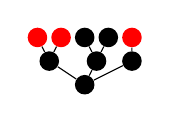
\begin{tikzpicture}[scale=.2]
\node[circle, scale=0.75, fill] (tid0) at (3.75,0){};
\node[circle, scale=0.75, fill] (tid1) at (1.5,1.5){};
\node[circle, scale=0.75, fill, red] (tid4) at (0.75,3){};
\node[circle, scale=0.75, fill, red] (tid5) at (2.25,3){};
\draw[](tid1) -- (tid4);
\draw[](tid1) -- (tid5);
\node[circle, scale=0.75, fill] (tid2) at (4.5,1.5){};
\node[circle, scale=0.75, fill] (tid6) at (3.75,3){};
\node[circle, scale=0.75, fill] (tid7) at (5.25,3){};
\draw[](tid2) -- (tid6);
\draw[](tid2) -- (tid7);
\node[circle, scale=0.75, fill] (tid3) at (6.75,1.5){};
\node[circle, scale=0.75, fill, red] (tid8) at (6.75,3){};
\draw[](tid3) -- (tid8);
\draw[](tid0) -- (tid1);
\draw[](tid0) -- (tid2);
\draw[](tid0) -- (tid3);

\end{tikzpicture}
\nodepart{two}
\footnotesize{4.87243}
\nodepart{three}
\footnotesize{0.67 0.33}
};
\node[draw=black, rectangle split, rectangle split parts=3] (sn0x92115d8W-27) at (-27, -36) {
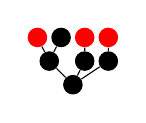
\begin{tikzpicture}[scale=.2]
\node[circle, scale=0.75, fill] (tid0) at (3,0){};
\node[circle, scale=0.75, fill] (tid1) at (1.5,1.5){};
\node[circle, scale=0.75, fill, red] (tid4) at (0.75,3){};
\node[circle, scale=0.75, fill] (tid5) at (2.25,3){};
\draw[](tid1) -- (tid4);
\draw[](tid1) -- (tid5);
\node[circle, scale=0.75, fill] (tid2) at (3.75,1.5){};
\node[circle, scale=0.75, fill, red] (tid6) at (3.75,3){};
\draw[](tid2) -- (tid6);
\node[circle, scale=0.75, fill] (tid3) at (5.25,1.5){};
\node[circle, scale=0.75, fill, red] (tid7) at (5.25,3){};
\draw[](tid3) -- (tid7);
\draw[](tid0) -- (tid1);
\draw[](tid0) -- (tid2);
\draw[](tid0) -- (tid3);

\end{tikzpicture}
\nodepart{two}
\footnotesize{4.54012}
\nodepart{three}
\footnotesize{0.33 0.67}
};
\node[draw=black, rectangle split, rectangle split parts=3] (sn0x920f510W-12) at (-12, -48) {
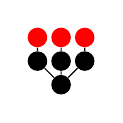
\begin{tikzpicture}[scale=.2]
\node[circle, scale=0.75, fill] (tid0) at (2.25,0){};
\node[circle, scale=0.75, fill] (tid1) at (0.75,1.5){};
\node[circle, scale=0.75, fill, red] (tid4) at (0.75,3){};
\draw[](tid1) -- (tid4);
\node[circle, scale=0.75, fill] (tid2) at (2.25,1.5){};
\node[circle, scale=0.75, fill, red] (tid5) at (2.25,3){};
\draw[](tid2) -- (tid5);
\node[circle, scale=0.75, fill] (tid3) at (3.75,1.5){};
\node[circle, scale=0.75, fill, red] (tid6) at (3.75,3){};
\draw[](tid3) -- (tid6);
\draw[](tid0) -- (tid1);
\draw[](tid0) -- (tid2);
\draw[](tid0) -- (tid3);

\end{tikzpicture}
\nodepart{two}
\footnotesize{4.21296}
\nodepart{three}
\footnotesize{1}
};
\node[draw=black, rectangle split, rectangle split parts=3] (sn0x9210968W-7) at (-7.25, -60) {
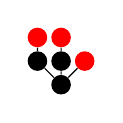
\begin{tikzpicture}[scale=.2]
\node[circle, scale=0.75, fill] (tid0) at (2.25,0){};
\node[circle, scale=0.75, fill] (tid1) at (0.75,1.5){};
\node[circle, scale=0.75, fill, red] (tid4) at (0.75,3){};
\draw[](tid1) -- (tid4);
\node[circle, scale=0.75, fill] (tid2) at (2.25,1.5){};
\node[circle, scale=0.75, fill, red] (tid5) at (2.25,3){};
\draw[](tid2) -- (tid5);
\node[circle, scale=0.75, fill, red] (tid3) at (3.75,1.5){};
\draw[](tid0) -- (tid1);
\draw[](tid0) -- (tid2);
\draw[](tid0) -- (tid3);

\end{tikzpicture}
\nodepart{two}
\footnotesize{3.87963}
\nodepart{three}
\footnotesize{0.33 0.67}
};
\node[draw=black, rectangle split, rectangle split parts=3] (sn0x9210b90W-9) at (-9, -72) {
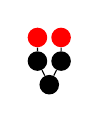
\begin{tikzpicture}[scale=.2]
\node[circle, scale=0.75, fill] (tid0) at (1.5,0){};
\node[circle, scale=0.75, fill] (tid1) at (0.75,1.5){};
\node[circle, scale=0.75, fill, red] (tid3) at (0.75,3){};
\draw[](tid1) -- (tid3);
\node[circle, scale=0.75, fill] (tid2) at (2.25,1.5){};
\node[circle, scale=0.75, fill, red] (tid4) at (2.25,3){};
\draw[](tid2) -- (tid4);
\draw[](tid0) -- (tid1);
\draw[](tid0) -- (tid2);

\end{tikzpicture}
\nodepart{two}
\footnotesize{3.75}
\nodepart{three}
\footnotesize{1}
};
\node[draw=black, rectangle split, rectangle split parts=3] (sn0x9210d88W-8) at (-8.25, -84) {
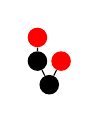
\begin{tikzpicture}[scale=.2]
\node[circle, scale=0.75, fill] (tid0) at (1.5,0){};
\node[circle, scale=0.75, fill] (tid1) at (0.75,1.5){};
\node[circle, scale=0.75, fill, red] (tid3) at (0.75,3){};
\draw[](tid1) -- (tid3);
\node[circle, scale=0.75, fill, red] (tid2) at (2.25,1.5){};
\draw[](tid0) -- (tid1);
\draw[](tid0) -- (tid2);

\end{tikzpicture}
\nodepart{two}
\footnotesize{3.25}
\nodepart{three}
\footnotesize{0.5 0.5}
};
\node[draw=black, rectangle split, rectangle split parts=3] (sn0x9210f38W-4) at (-4.25, -96) {
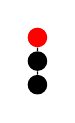
\begin{tikzpicture}[scale=.2]
\node[circle, scale=0.75, fill] (tid0) at (0.75,0){};
\node[circle, scale=0.75, fill] (tid1) at (0.75,1.5){};
\node[circle, scale=0.75, fill, red] (tid2) at (0.75,3){};
\draw[](tid1) -- (tid2);
\draw[](tid0) -- (tid1);

\end{tikzpicture}
\nodepart{two}
\footnotesize{3}
\nodepart{three}
\footnotesize{1}
};
\node[draw=black, rectangle split, rectangle split parts=3] (sn0x9211160W-1) at (-1.75, -108) {

\begin{tikzpicture}[scale=.2]
\node[circle, scale=0.75, fill] (tid0) at (0.75,0){};
\node[circle, scale=0.75, fill, red] (tid1) at (0.75,1.5){};
\draw[](tid0) -- (tid1);

\end{tikzpicture}
\nodepart{two}
\footnotesize{2}
\nodepart{three}
\footnotesize{1}
};
\node[draw=black, rectangle split, rectangle split parts=3] (sn0x92111d8W-1) at (-1.75, -120) {

\begin{tikzpicture}[scale=.2]
\node[circle, scale=0.75, fill, red] (tid0) at (0.75,0){};

\end{tikzpicture}
\nodepart{two}
\footnotesize{1}
\nodepart{three}
\footnotesize{}
};
\draw (sn0x9211160W-1.south) -- (sn0x92111d8W-1.north);
\draw (sn0x9210f38W-4.south) -- (sn0x9211160W-1.north);
\node[draw=black, rectangle split, rectangle split parts=3] (sn0x9210fa0W0) at (-0.75, -96) {

\begin{tikzpicture}[scale=.2]
\node[circle, scale=0.75, fill] (tid0) at (1.5,0){};
\node[circle, scale=0.75, fill, red] (tid1) at (0.75,1.5){};
\node[circle, scale=0.75, fill, red] (tid2) at (2.25,1.5){};
\draw[](tid0) -- (tid1);
\draw[](tid0) -- (tid2);

\end{tikzpicture}
\nodepart{two}
\footnotesize{2.5}
\nodepart{three}
\footnotesize{1}
};
\draw (sn0x9210fa0W0.south) -- (sn0x9211160W-1.north);
\draw (sn0x9210d88W-8.south) -- (sn0x9210f38W-4.north);
\draw (sn0x9210d88W-8.south) -- (sn0x9210fa0W0.north);
\draw (sn0x9210b90W-9.south) -- (sn0x9210d88W-8.north);
\node[draw=black, rectangle split, rectangle split parts=3] (sn0x9210c28W-4) at (-4, -72) {
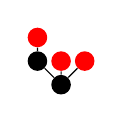
\begin{tikzpicture}[scale=.2]
\node[circle, scale=0.75, fill] (tid0) at (2.25,0){};
\node[circle, scale=0.75, fill] (tid1) at (0.75,1.5){};
\node[circle, scale=0.75, fill, red] (tid4) at (0.75,3){};
\draw[](tid1) -- (tid4);
\node[circle, scale=0.75, fill, red] (tid2) at (2.25,1.5){};
\node[circle, scale=0.75, fill, red] (tid3) at (3.75,1.5){};
\draw[](tid0) -- (tid1);
\draw[](tid0) -- (tid2);
\draw[](tid0) -- (tid3);

\end{tikzpicture}
\nodepart{two}
\footnotesize{3.44444}
\nodepart{three}
\footnotesize{0.67 0.33}
};
\node[draw=black, rectangle split, rectangle split parts=3] (sn0x9215aa8W-3) at (-3.25, -84) {
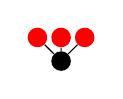
\begin{tikzpicture}[scale=.2]
\node[circle, scale=0.75, fill] (tid0) at (2.25,0){};
\node[circle, scale=0.75, fill, red] (tid1) at (0.75,1.5){};
\node[circle, scale=0.75, fill, red] (tid2) at (2.25,1.5){};
\node[circle, scale=0.75, fill, red] (tid3) at (3.75,1.5){};
\draw[](tid0) -- (tid1);
\draw[](tid0) -- (tid2);
\draw[](tid0) -- (tid3);

\end{tikzpicture}
\nodepart{two}
\footnotesize{2.83333}
\nodepart{three}
\footnotesize{1}
};
\draw (sn0x9215aa8W-3.south) -- (sn0x9210fa0W0.north);
\draw (sn0x9210c28W-4.south) -- (sn0x9210d88W-8.north);
\draw (sn0x9210c28W-4.south) -- (sn0x9215aa8W-3.north);
\draw (sn0x9210968W-7.south) -- (sn0x9210b90W-9.north);
\draw (sn0x9210968W-7.south) -- (sn0x9210c28W-4.north);
\draw (sn0x920f510W-12.south) -- (sn0x9210968W-7.north);
\node[draw=black, rectangle split, rectangle split parts=3] (sn0x92105f0W-5) at (-5.5, -48) {
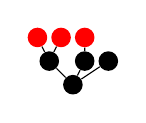
\begin{tikzpicture}[scale=.2]
\node[circle, scale=0.75, fill] (tid0) at (3,0){};
\node[circle, scale=0.75, fill] (tid1) at (1.5,1.5){};
\node[circle, scale=0.75, fill, red] (tid4) at (0.75,3){};
\node[circle, scale=0.75, fill, red] (tid5) at (2.25,3){};
\draw[](tid1) -- (tid4);
\draw[](tid1) -- (tid5);
\node[circle, scale=0.75, fill] (tid2) at (3.75,1.5){};
\node[circle, scale=0.75, fill, red] (tid6) at (3.75,3){};
\draw[](tid2) -- (tid6);
\node[circle, scale=0.75, fill] (tid3) at (5.25,1.5){};
\draw[](tid0) -- (tid1);
\draw[](tid0) -- (tid2);
\draw[](tid0) -- (tid3);

\end{tikzpicture}
\nodepart{two}
\footnotesize{4.2037}
\nodepart{three}
\footnotesize{0.67 0.33}
};
\node[draw=black, rectangle split, rectangle split parts=3] (sn0x9215e90W0) at (-0.75, -60) {
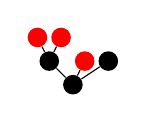
\begin{tikzpicture}[scale=.2]
\node[circle, scale=0.75, fill] (tid0) at (3,0){};
\node[circle, scale=0.75, fill] (tid1) at (1.5,1.5){};
\node[circle, scale=0.75, fill, red] (tid4) at (0.75,3){};
\node[circle, scale=0.75, fill, red] (tid5) at (2.25,3){};
\draw[](tid1) -- (tid4);
\draw[](tid1) -- (tid5);
\node[circle, scale=0.75, fill, red] (tid2) at (3.75,1.5){};
\node[circle, scale=0.75, fill] (tid3) at (5.25,1.5){};
\draw[](tid0) -- (tid1);
\draw[](tid0) -- (tid2);
\draw[](tid0) -- (tid3);

\end{tikzpicture}
\nodepart{two}
\footnotesize{3.85185}
\nodepart{three}
\footnotesize{0.33 0.67}
};
\node[draw=black, rectangle split, rectangle split parts=3] (sn0x9216188W2) at (2.5, -72) {
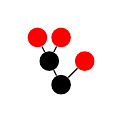
\begin{tikzpicture}[scale=.2]
\node[circle, scale=0.75, fill] (tid0) at (2.25,0){};
\node[circle, scale=0.75, fill] (tid1) at (1.5,1.5){};
\node[circle, scale=0.75, fill, red] (tid3) at (0.75,3){};
\node[circle, scale=0.75, fill, red] (tid4) at (2.25,3){};
\draw[](tid1) -- (tid3);
\draw[](tid1) -- (tid4);
\node[circle, scale=0.75, fill, red] (tid2) at (3.75,1.5){};
\draw[](tid0) -- (tid1);
\draw[](tid0) -- (tid2);

\end{tikzpicture}
\nodepart{two}
\footnotesize{3.66667}
\nodepart{three}
\footnotesize{0.33 0.67}
};
\node[draw=black, rectangle split, rectangle split parts=3] (sn0x9215c40W3) at (3.25, -84) {
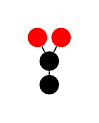
\begin{tikzpicture}[scale=.2]
\node[circle, scale=0.75, fill] (tid0) at (1.5,0){};
\node[circle, scale=0.75, fill] (tid1) at (1.5,1.5){};
\node[circle, scale=0.75, fill, red] (tid2) at (0.75,3){};
\node[circle, scale=0.75, fill, red] (tid3) at (2.25,3){};
\draw[](tid1) -- (tid2);
\draw[](tid1) -- (tid3);
\draw[](tid0) -- (tid1);

\end{tikzpicture}
\nodepart{two}
\footnotesize{3.5}
\nodepart{three}
\footnotesize{1}
};
\draw (sn0x9215c40W3.south) -- (sn0x9210f38W-4.north);
\draw (sn0x9216188W2.south) -- (sn0x9215c40W3.north);
\draw (sn0x9216188W2.south) -- (sn0x9210d88W-8.north);
\draw (sn0x9215e90W0.south) -- (sn0x9216188W2.north);
\draw (sn0x9215e90W0.south) -- (sn0x9210c28W-4.north);
\draw (sn0x92105f0W-5.south) -- (sn0x9210968W-7.north);
\draw (sn0x92105f0W-5.south) -- (sn0x9215e90W0.north);
\draw (sn0x92115d8W-27.south) -- (sn0x920f510W-12.north);
\draw (sn0x92115d8W-27.south) -- (sn0x92105f0W-5.north);
\node[draw=black, rectangle split, rectangle split parts=3] (sn0x9215cf0W-19) at (-19, -36) {
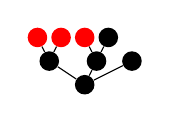
\begin{tikzpicture}[scale=.2]
\node[circle, scale=0.75, fill] (tid0) at (3.75,0){};
\node[circle, scale=0.75, fill] (tid1) at (1.5,1.5){};
\node[circle, scale=0.75, fill, red] (tid4) at (0.75,3){};
\node[circle, scale=0.75, fill, red] (tid5) at (2.25,3){};
\draw[](tid1) -- (tid4);
\draw[](tid1) -- (tid5);
\node[circle, scale=0.75, fill] (tid2) at (4.5,1.5){};
\node[circle, scale=0.75, fill, red] (tid6) at (3.75,3){};
\node[circle, scale=0.75, fill] (tid7) at (5.25,3){};
\draw[](tid2) -- (tid6);
\draw[](tid2) -- (tid7);
\node[circle, scale=0.75, fill] (tid3) at (6.75,1.5){};
\draw[](tid0) -- (tid1);
\draw[](tid0) -- (tid2);
\draw[](tid0) -- (tid3);

\end{tikzpicture}
\nodepart{two}
\footnotesize{4.53704}
\nodepart{three}
\footnotesize{1}
};
\draw (sn0x9215cf0W-19.south) -- (sn0x92105f0W-5.north);
\draw (sn0x9217928W-20.south) -- (sn0x92115d8W-27.north);
\draw (sn0x9217928W-20.south) -- (sn0x9215cf0W-19.north);
\node[draw=black, rectangle split, rectangle split parts=3] (sn0x920f210W-11) at (-11, -24) {
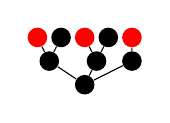
\begin{tikzpicture}[scale=.2]
\node[circle, scale=0.75, fill] (tid0) at (3.75,0){};
\node[circle, scale=0.75, fill] (tid1) at (1.5,1.5){};
\node[circle, scale=0.75, fill, red] (tid4) at (0.75,3){};
\node[circle, scale=0.75, fill] (tid5) at (2.25,3){};
\draw[](tid1) -- (tid4);
\draw[](tid1) -- (tid5);
\node[circle, scale=0.75, fill] (tid2) at (4.5,1.5){};
\node[circle, scale=0.75, fill, red] (tid6) at (3.75,3){};
\node[circle, scale=0.75, fill] (tid7) at (5.25,3){};
\draw[](tid2) -- (tid6);
\draw[](tid2) -- (tid7);
\node[circle, scale=0.75, fill] (tid3) at (6.75,1.5){};
\node[circle, scale=0.75, fill, red] (tid8) at (6.75,3){};
\draw[](tid3) -- (tid8);
\draw[](tid0) -- (tid1);
\draw[](tid0) -- (tid2);
\draw[](tid0) -- (tid3);

\end{tikzpicture}
\nodepart{two}
\footnotesize{4.87346}
\nodepart{three}
\footnotesize{0.33 0.33 0.17 0.17}
};
\node[draw=black, rectangle split, rectangle split parts=3] (sn0x920f478W-9) at (-9.5, -36) {
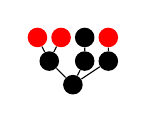
\begin{tikzpicture}[scale=.2]
\node[circle, scale=0.75, fill] (tid0) at (3,0){};
\node[circle, scale=0.75, fill] (tid1) at (1.5,1.5){};
\node[circle, scale=0.75, fill, red] (tid4) at (0.75,3){};
\node[circle, scale=0.75, fill, red] (tid5) at (2.25,3){};
\draw[](tid1) -- (tid4);
\draw[](tid1) -- (tid5);
\node[circle, scale=0.75, fill] (tid2) at (3.75,1.5){};
\node[circle, scale=0.75, fill] (tid6) at (3.75,3){};
\draw[](tid2) -- (tid6);
\node[circle, scale=0.75, fill] (tid3) at (5.25,1.5){};
\node[circle, scale=0.75, fill, red] (tid7) at (5.25,3){};
\draw[](tid3) -- (tid7);
\draw[](tid0) -- (tid1);
\draw[](tid0) -- (tid2);
\draw[](tid0) -- (tid3);

\end{tikzpicture}
\nodepart{two}
\footnotesize{4.54321}
\nodepart{three}
\footnotesize{0.67 0.33}
};
\draw (sn0x920f478W-9.south) -- (sn0x920f510W-12.north);
\draw (sn0x920f478W-9.south) -- (sn0x92105f0W-5.north);
\node[draw=black, rectangle split, rectangle split parts=3] (sn0x9216a40W-1) at (-1.5, -36) {
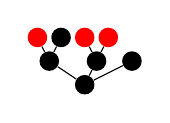
\begin{tikzpicture}[scale=.2]
\node[circle, scale=0.75, fill] (tid0) at (3.75,0){};
\node[circle, scale=0.75, fill] (tid1) at (1.5,1.5){};
\node[circle, scale=0.75, fill, red] (tid4) at (0.75,3){};
\node[circle, scale=0.75, fill] (tid5) at (2.25,3){};
\draw[](tid1) -- (tid4);
\draw[](tid1) -- (tid5);
\node[circle, scale=0.75, fill] (tid2) at (4.5,1.5){};
\node[circle, scale=0.75, fill, red] (tid6) at (3.75,3){};
\node[circle, scale=0.75, fill, red] (tid7) at (5.25,3){};
\draw[](tid2) -- (tid6);
\draw[](tid2) -- (tid7);
\node[circle, scale=0.75, fill] (tid3) at (6.75,1.5){};
\draw[](tid0) -- (tid1);
\draw[](tid0) -- (tid2);
\draw[](tid0) -- (tid3);

\end{tikzpicture}
\nodepart{two}
\footnotesize{4.53704}
\nodepart{three}
\footnotesize{1}
};
\draw (sn0x9216a40W-1.south) -- (sn0x92105f0W-5.north);
\draw (sn0x920f210W-11.south) -- (sn0x92115d8W-27.north);
\draw (sn0x920f210W-11.south) -- (sn0x920f478W-9.north);
\draw (sn0x920f210W-11.south) -- (sn0x9215cf0W-19.north);
\draw (sn0x920f210W-11.south) -- (sn0x9216a40W-1.north);
\node[draw=black, rectangle split, rectangle split parts=3] (sn0x9217aa0W-1) at (-1.5, -24) {
\begin{tikzpicture}[scale=.2]
\node[circle, scale=0.75, fill] (tid0) at (4.5,0){};
\node[circle, scale=0.75, fill] (tid1) at (2.25,1.5){};
\node[circle, scale=0.75, fill, red] (tid4) at (0.75,3){};
\node[circle, scale=0.75, fill, red] (tid5) at (2.25,3){};
\node[circle, scale=0.75, fill, red] (tid6) at (3.75,3){};
\draw[](tid1) -- (tid4);
\draw[](tid1) -- (tid5);
\draw[](tid1) -- (tid6);
\node[circle, scale=0.75, fill] (tid2) at (6,1.5){};
\node[circle, scale=0.75, fill] (tid7) at (5.25,3){};
\node[circle, scale=0.75, fill] (tid8) at (6.75,3){};
\draw[](tid2) -- (tid7);
\draw[](tid2) -- (tid8);
\node[circle, scale=0.75, fill] (tid3) at (8.25,1.5){};
\draw[](tid0) -- (tid1);
\draw[](tid0) -- (tid2);
\draw[](tid0) -- (tid3);

\end{tikzpicture}
\nodepart{two}
\footnotesize{4.87037}
\nodepart{three}
\footnotesize{1}
};
\draw (sn0x9217aa0W-1.south) -- (sn0x9215cf0W-19.north);
\node[draw=black, rectangle split, rectangle split parts=3] (sn0x9217ee0W9) at (9.5, -24) {
\begin{tikzpicture}[scale=.2]
\node[circle, scale=0.75, fill] (tid0) at (4.5,0){};
\node[circle, scale=0.75, fill] (tid1) at (2.25,1.5){};
\node[circle, scale=0.75, fill, red] (tid4) at (0.75,3){};
\node[circle, scale=0.75, fill, red] (tid5) at (2.25,3){};
\node[circle, scale=0.75, fill] (tid6) at (3.75,3){};
\draw[](tid1) -- (tid4);
\draw[](tid1) -- (tid5);
\draw[](tid1) -- (tid6);
\node[circle, scale=0.75, fill] (tid2) at (6,1.5){};
\node[circle, scale=0.75, fill, red] (tid7) at (5.25,3){};
\node[circle, scale=0.75, fill] (tid8) at (6.75,3){};
\draw[](tid2) -- (tid7);
\draw[](tid2) -- (tid8);
\node[circle, scale=0.75, fill] (tid3) at (8.25,1.5){};
\draw[](tid0) -- (tid1);
\draw[](tid0) -- (tid2);
\draw[](tid0) -- (tid3);

\end{tikzpicture}
\nodepart{two}
\footnotesize{4.86934}
\nodepart{three}
\footnotesize{0.33 0.33 0.17 0.17}
};
\node[draw=black, rectangle split, rectangle split parts=3] (sn0x9216c00W8) at (8, -36) {
\begin{tikzpicture}[scale=.2]
\node[circle, scale=0.75, fill] (tid0) at (3.75,0){};
\node[circle, scale=0.75, fill] (tid1) at (2.25,1.5){};
\node[circle, scale=0.75, fill, red] (tid4) at (0.75,3){};
\node[circle, scale=0.75, fill, red] (tid5) at (2.25,3){};
\node[circle, scale=0.75, fill, red] (tid6) at (3.75,3){};
\draw[](tid1) -- (tid4);
\draw[](tid1) -- (tid5);
\draw[](tid1) -- (tid6);
\node[circle, scale=0.75, fill] (tid2) at (5.25,1.5){};
\node[circle, scale=0.75, fill] (tid7) at (5.25,3){};
\draw[](tid2) -- (tid7);
\node[circle, scale=0.75, fill] (tid3) at (6.75,1.5){};
\draw[](tid0) -- (tid1);
\draw[](tid0) -- (tid2);
\draw[](tid0) -- (tid3);

\end{tikzpicture}
\nodepart{two}
\footnotesize{4.53704}
\nodepart{three}
\footnotesize{1}
};
\draw (sn0x9216c00W8.south) -- (sn0x92105f0W-5.north);
\node[draw=black, rectangle split, rectangle split parts=3] (sn0x9217040W17) at (17.5, -36) {
\begin{tikzpicture}[scale=.2]
\node[circle, scale=0.75, fill] (tid0) at (3.75,0){};
\node[circle, scale=0.75, fill] (tid1) at (2.25,1.5){};
\node[circle, scale=0.75, fill, red] (tid4) at (0.75,3){};
\node[circle, scale=0.75, fill, red] (tid5) at (2.25,3){};
\node[circle, scale=0.75, fill] (tid6) at (3.75,3){};
\draw[](tid1) -- (tid4);
\draw[](tid1) -- (tid5);
\draw[](tid1) -- (tid6);
\node[circle, scale=0.75, fill] (tid2) at (5.25,1.5){};
\node[circle, scale=0.75, fill, red] (tid7) at (5.25,3){};
\draw[](tid2) -- (tid7);
\node[circle, scale=0.75, fill] (tid3) at (6.75,1.5){};
\draw[](tid0) -- (tid1);
\draw[](tid0) -- (tid2);
\draw[](tid0) -- (tid3);

\end{tikzpicture}
\nodepart{two}
\footnotesize{4.53086}
\nodepart{three}
\footnotesize{0.67 0.33}
};
\node[draw=black, rectangle split, rectangle split parts=3] (sn0x9217148W2) at (2.5, -48) {
\begin{tikzpicture}[scale=.2]
\node[circle, scale=0.75, fill] (tid0) at (3.75,0){};
\node[circle, scale=0.75, fill] (tid1) at (2.25,1.5){};
\node[circle, scale=0.75, fill, red] (tid4) at (0.75,3){};
\node[circle, scale=0.75, fill, red] (tid5) at (2.25,3){};
\node[circle, scale=0.75, fill, red] (tid6) at (3.75,3){};
\draw[](tid1) -- (tid4);
\draw[](tid1) -- (tid5);
\draw[](tid1) -- (tid6);
\node[circle, scale=0.75, fill] (tid2) at (5.25,1.5){};
\node[circle, scale=0.75, fill] (tid3) at (6.75,1.5){};
\draw[](tid0) -- (tid1);
\draw[](tid0) -- (tid2);
\draw[](tid0) -- (tid3);

\end{tikzpicture}
\nodepart{two}
\footnotesize{4.18519}
\nodepart{three}
\footnotesize{1}
};
\draw (sn0x9217148W2.south) -- (sn0x9215e90W0.north);
\draw (sn0x9217040W17.south) -- (sn0x92105f0W-5.north);
\draw (sn0x9217040W17.south) -- (sn0x9217148W2.north);
\draw (sn0x9217ee0W9.south) -- (sn0x9215cf0W-19.north);
\draw (sn0x9217ee0W9.south) -- (sn0x9216a40W-1.north);
\draw (sn0x9217ee0W9.south) -- (sn0x9216c00W8.north);
\draw (sn0x9217ee0W9.south) -- (sn0x9217040W17.north);
\draw (sn0x920fcc0W-5.south) -- (sn0x9217928W-20.north);
\draw (sn0x920fcc0W-5.south) -- (sn0x920f210W-11.north);
\draw (sn0x920fcc0W-5.south) -- (sn0x9217aa0W-1.north);
\draw (sn0x920fcc0W-5.south) -- (sn0x9217ee0W9.north);
\end{tikzpicture}

%%% Local Variables:
%%% TeX-master: "thesis/thesis.tex"
%%% End: 

\begin{tikzpicture}[scale=.2, anchor=south west]
\node[draw=black, rectangle split, rectangle split parts=3] (sn0x920fd20W-5) at (-5.5, -12) {
\begin{tikzpicture}[scale=.2]
\node[circle, scale=0.75, fill] (tid0) at (4.5,0){};
\node[circle, scale=0.75, fill] (tid1) at (2.25,1.5){};
\node[circle, scale=0.75, fill, red] (tid4) at (0.75,3){};
\node[circle, scale=0.75, fill, red] (tid5) at (2.25,3){};
\node[circle, scale=0.75, fill, red] (tid6) at (3.75,3){};
\draw[](tid1) -- (tid4);
\draw[](tid1) -- (tid5);
\draw[](tid1) -- (tid6);
\node[circle, scale=0.75, fill] (tid2) at (6,1.5){};
\node[circle, scale=0.75, fill] (tid7) at (5.25,3){};
\node[circle, scale=0.75, fill] (tid8) at (6.75,3){};
\draw[](tid2) -- (tid7);
\draw[](tid2) -- (tid8);
\node[circle, scale=0.75, fill] (tid3) at (8.25,1.5){};
\node[circle, scale=0.75, fill] (tid9) at (8.25,3){};
\draw[](tid3) -- (tid9);
\draw[](tid0) -- (tid1);
\draw[](tid0) -- (tid2);
\draw[](tid0) -- (tid3);

\end{tikzpicture}
\nodepart{two}
\footnotesize{5.20782}
\nodepart{three}
\footnotesize{0.67 0.33}
};
\node[draw=black, rectangle split, rectangle split parts=3] (sn0x920e170W-9) at (-9.5, -24) {
\begin{tikzpicture}[scale=.2]
\node[circle, scale=0.75, fill] (tid0) at (3.75,0){};
\node[circle, scale=0.75, fill] (tid1) at (1.5,1.5){};
\node[circle, scale=0.75, fill, red] (tid4) at (0.75,3){};
\node[circle, scale=0.75, fill, red] (tid5) at (2.25,3){};
\draw[](tid1) -- (tid4);
\draw[](tid1) -- (tid5);
\node[circle, scale=0.75, fill] (tid2) at (4.5,1.5){};
\node[circle, scale=0.75, fill, red] (tid6) at (3.75,3){};
\node[circle, scale=0.75, fill] (tid7) at (5.25,3){};
\draw[](tid2) -- (tid6);
\draw[](tid2) -- (tid7);
\node[circle, scale=0.75, fill] (tid3) at (6.75,1.5){};
\node[circle, scale=0.75, fill] (tid8) at (6.75,3){};
\draw[](tid3) -- (tid8);
\draw[](tid0) -- (tid1);
\draw[](tid0) -- (tid2);
\draw[](tid0) -- (tid3);

\end{tikzpicture}
\nodepart{two}
\footnotesize{4.87551}
\nodepart{three}
\footnotesize{0.5 0.33 0.17}
};
\node[draw=black, rectangle split, rectangle split parts=3] (sn0x9211948W-16) at (-16.75, -36) {
\begin{tikzpicture}[scale=.2]
\node[circle, scale=0.75, fill] (tid0) at (3,0){};
\node[circle, scale=0.75, fill] (tid1) at (1.5,1.5){};
\node[circle, scale=0.75, fill, red] (tid4) at (0.75,3){};
\node[circle, scale=0.75, fill, red] (tid5) at (2.25,3){};
\draw[](tid1) -- (tid4);
\draw[](tid1) -- (tid5);
\node[circle, scale=0.75, fill] (tid2) at (3.75,1.5){};
\node[circle, scale=0.75, fill, red] (tid6) at (3.75,3){};
\draw[](tid2) -- (tid6);
\node[circle, scale=0.75, fill] (tid3) at (5.25,1.5){};
\node[circle, scale=0.75, fill] (tid7) at (5.25,3){};
\draw[](tid3) -- (tid7);
\draw[](tid0) -- (tid1);
\draw[](tid0) -- (tid2);
\draw[](tid0) -- (tid3);

\end{tikzpicture}
\nodepart{two}
\footnotesize{4.54321}
\nodepart{three}
\footnotesize{0.67 0.33}
};
\node[draw=black, rectangle split, rectangle split parts=3] (sn0x920f510W-7) at (-7.25, -48) {
\begin{tikzpicture}[scale=.2]
\node[circle, scale=0.75, fill] (tid0) at (2.25,0){};
\node[circle, scale=0.75, fill] (tid1) at (0.75,1.5){};
\node[circle, scale=0.75, fill, red] (tid4) at (0.75,3){};
\draw[](tid1) -- (tid4);
\node[circle, scale=0.75, fill] (tid2) at (2.25,1.5){};
\node[circle, scale=0.75, fill, red] (tid5) at (2.25,3){};
\draw[](tid2) -- (tid5);
\node[circle, scale=0.75, fill] (tid3) at (3.75,1.5){};
\node[circle, scale=0.75, fill, red] (tid6) at (3.75,3){};
\draw[](tid3) -- (tid6);
\draw[](tid0) -- (tid1);
\draw[](tid0) -- (tid2);
\draw[](tid0) -- (tid3);

\end{tikzpicture}
\nodepart{two}
\footnotesize{4.21296}
\nodepart{three}
\footnotesize{1}
};
\node[draw=black, rectangle split, rectangle split parts=3] (sn0x9210968W-7) at (-7.25, -60) {
\begin{tikzpicture}[scale=.2]
\node[circle, scale=0.75, fill] (tid0) at (2.25,0){};
\node[circle, scale=0.75, fill] (tid1) at (0.75,1.5){};
\node[circle, scale=0.75, fill, red] (tid4) at (0.75,3){};
\draw[](tid1) -- (tid4);
\node[circle, scale=0.75, fill] (tid2) at (2.25,1.5){};
\node[circle, scale=0.75, fill, red] (tid5) at (2.25,3){};
\draw[](tid2) -- (tid5);
\node[circle, scale=0.75, fill, red] (tid3) at (3.75,1.5){};
\draw[](tid0) -- (tid1);
\draw[](tid0) -- (tid2);
\draw[](tid0) -- (tid3);

\end{tikzpicture}
\nodepart{two}
\footnotesize{3.87963}
\nodepart{three}
\footnotesize{0.33 0.67}
};
\node[draw=black, rectangle split, rectangle split parts=3] (sn0x9210b90W-9) at (-9, -72) {
\begin{tikzpicture}[scale=.2]
\node[circle, scale=0.75, fill] (tid0) at (1.5,0){};
\node[circle, scale=0.75, fill] (tid1) at (0.75,1.5){};
\node[circle, scale=0.75, fill, red] (tid3) at (0.75,3){};
\draw[](tid1) -- (tid3);
\node[circle, scale=0.75, fill] (tid2) at (2.25,1.5){};
\node[circle, scale=0.75, fill, red] (tid4) at (2.25,3){};
\draw[](tid2) -- (tid4);
\draw[](tid0) -- (tid1);
\draw[](tid0) -- (tid2);

\end{tikzpicture}
\nodepart{two}
\footnotesize{3.75}
\nodepart{three}
\footnotesize{1}
};
\node[draw=black, rectangle split, rectangle split parts=3] (sn0x9210d88W-8) at (-8.25, -84) {
\begin{tikzpicture}[scale=.2]
\node[circle, scale=0.75, fill] (tid0) at (1.5,0){};
\node[circle, scale=0.75, fill] (tid1) at (0.75,1.5){};
\node[circle, scale=0.75, fill, red] (tid3) at (0.75,3){};
\draw[](tid1) -- (tid3);
\node[circle, scale=0.75, fill, red] (tid2) at (2.25,1.5){};
\draw[](tid0) -- (tid1);
\draw[](tid0) -- (tid2);

\end{tikzpicture}
\nodepart{two}
\footnotesize{3.25}
\nodepart{three}
\footnotesize{0.5 0.5}
};
\node[draw=black, rectangle split, rectangle split parts=3] (sn0x9210f38W-4) at (-4.25, -96) {
\begin{tikzpicture}[scale=.2]
\node[circle, scale=0.75, fill] (tid0) at (0.75,0){};
\node[circle, scale=0.75, fill] (tid1) at (0.75,1.5){};
\node[circle, scale=0.75, fill, red] (tid2) at (0.75,3){};
\draw[](tid1) -- (tid2);
\draw[](tid0) -- (tid1);

\end{tikzpicture}
\nodepart{two}
\footnotesize{3}
\nodepart{three}
\footnotesize{1}
};
\node[draw=black, rectangle split, rectangle split parts=3] (sn0x9211160W-1) at (-1.75, -108) {
\begin{tikzpicture}[scale=.2]
\node[circle, scale=0.75, fill] (tid0) at (0.75,0){};
\node[circle, scale=0.75, fill, red] (tid1) at (0.75,1.5){};
\draw[](tid0) -- (tid1);

\end{tikzpicture}
\nodepart{two}
\footnotesize{2}
\nodepart{three}
\footnotesize{1}
};
\node[draw=black, rectangle split, rectangle split parts=3] (sn0x92111d8W-1) at (-1.75, -120) {
\begin{tikzpicture}[scale=.2]
\node[circle, scale=0.75, fill, red] (tid0) at (0.75,0){};

\end{tikzpicture}
\nodepart{two}
\footnotesize{1}
\nodepart{three}
\footnotesize{}
};
\draw (sn0x9211160W-1.south) -- (sn0x92111d8W-1.north);
\draw (sn0x9210f38W-4.south) -- (sn0x9211160W-1.north);
\node[draw=black, rectangle split, rectangle split parts=3] (sn0x9210fa0W0) at (-0.75, -96) {
\begin{tikzpicture}[scale=.2]
\node[circle, scale=0.75, fill] (tid0) at (1.5,0){};
\node[circle, scale=0.75, fill, red] (tid1) at (0.75,1.5){};
\node[circle, scale=0.75, fill, red] (tid2) at (2.25,1.5){};
\draw[](tid0) -- (tid1);
\draw[](tid0) -- (tid2);

\end{tikzpicture}
\nodepart{two}
\footnotesize{2.5}
\nodepart{three}
\footnotesize{1}
};
\draw (sn0x9210fa0W0.south) -- (sn0x9211160W-1.north);
\draw (sn0x9210d88W-8.south) -- (sn0x9210f38W-4.north);
\draw (sn0x9210d88W-8.south) -- (sn0x9210fa0W0.north);
\draw (sn0x9210b90W-9.south) -- (sn0x9210d88W-8.north);
\node[draw=black, rectangle split, rectangle split parts=3] (sn0x9210c28W-4) at (-4, -72) {
\begin{tikzpicture}[scale=.2]
\node[circle, scale=0.75, fill] (tid0) at (2.25,0){};
\node[circle, scale=0.75, fill] (tid1) at (0.75,1.5){};
\node[circle, scale=0.75, fill, red] (tid4) at (0.75,3){};
\draw[](tid1) -- (tid4);
\node[circle, scale=0.75, fill, red] (tid2) at (2.25,1.5){};
\node[circle, scale=0.75, fill, red] (tid3) at (3.75,1.5){};
\draw[](tid0) -- (tid1);
\draw[](tid0) -- (tid2);
\draw[](tid0) -- (tid3);

\end{tikzpicture}
\nodepart{two}
\footnotesize{3.44444}
\nodepart{three}
\footnotesize{0.67 0.33}
};
\node[draw=black, rectangle split, rectangle split parts=3] (sn0x9215aa8W-3) at (-3.25, -84) {
\begin{tikzpicture}[scale=.2]
\node[circle, scale=0.75, fill] (tid0) at (2.25,0){};
\node[circle, scale=0.75, fill, red] (tid1) at (0.75,1.5){};
\node[circle, scale=0.75, fill, red] (tid2) at (2.25,1.5){};
\node[circle, scale=0.75, fill, red] (tid3) at (3.75,1.5){};
\draw[](tid0) -- (tid1);
\draw[](tid0) -- (tid2);
\draw[](tid0) -- (tid3);

\end{tikzpicture}
\nodepart{two}
\footnotesize{2.83333}
\nodepart{three}
\footnotesize{1}
};
\draw (sn0x9215aa8W-3.south) -- (sn0x9210fa0W0.north);
\draw (sn0x9210c28W-4.south) -- (sn0x9210d88W-8.north);
\draw (sn0x9210c28W-4.south) -- (sn0x9215aa8W-3.north);
\draw (sn0x9210968W-7.south) -- (sn0x9210b90W-9.north);
\draw (sn0x9210968W-7.south) -- (sn0x9210c28W-4.north);
\draw (sn0x920f510W-7.south) -- (sn0x9210968W-7.north);
\node[draw=black, rectangle split, rectangle split parts=3] (sn0x92105f0W0) at (-0.75, -48) {
\begin{tikzpicture}[scale=.2]
\node[circle, scale=0.75, fill] (tid0) at (3,0){};
\node[circle, scale=0.75, fill] (tid1) at (1.5,1.5){};
\node[circle, scale=0.75, fill, red] (tid4) at (0.75,3){};
\node[circle, scale=0.75, fill, red] (tid5) at (2.25,3){};
\draw[](tid1) -- (tid4);
\draw[](tid1) -- (tid5);
\node[circle, scale=0.75, fill] (tid2) at (3.75,1.5){};
\node[circle, scale=0.75, fill, red] (tid6) at (3.75,3){};
\draw[](tid2) -- (tid6);
\node[circle, scale=0.75, fill] (tid3) at (5.25,1.5){};
\draw[](tid0) -- (tid1);
\draw[](tid0) -- (tid2);
\draw[](tid0) -- (tid3);

\end{tikzpicture}
\nodepart{two}
\footnotesize{4.2037}
\nodepart{three}
\footnotesize{0.67 0.33}
};
\node[draw=black, rectangle split, rectangle split parts=3] (sn0x9215e90W0) at (-0.75, -60) {
\begin{tikzpicture}[scale=.2]
\node[circle, scale=0.75, fill] (tid0) at (3,0){};
\node[circle, scale=0.75, fill] (tid1) at (1.5,1.5){};
\node[circle, scale=0.75, fill, red] (tid4) at (0.75,3){};
\node[circle, scale=0.75, fill, red] (tid5) at (2.25,3){};
\draw[](tid1) -- (tid4);
\draw[](tid1) -- (tid5);
\node[circle, scale=0.75, fill, red] (tid2) at (3.75,1.5){};
\node[circle, scale=0.75, fill] (tid3) at (5.25,1.5){};
\draw[](tid0) -- (tid1);
\draw[](tid0) -- (tid2);
\draw[](tid0) -- (tid3);

\end{tikzpicture}
\nodepart{two}
\footnotesize{3.85185}
\nodepart{three}
\footnotesize{0.33 0.67}
};
\node[draw=black, rectangle split, rectangle split parts=3] (sn0x9216188W2) at (2.5, -72) {
\begin{tikzpicture}[scale=.2]
\node[circle, scale=0.75, fill] (tid0) at (2.25,0){};
\node[circle, scale=0.75, fill] (tid1) at (1.5,1.5){};
\node[circle, scale=0.75, fill, red] (tid3) at (0.75,3){};
\node[circle, scale=0.75, fill, red] (tid4) at (2.25,3){};
\draw[](tid1) -- (tid3);
\draw[](tid1) -- (tid4);
\node[circle, scale=0.75, fill, red] (tid2) at (3.75,1.5){};
\draw[](tid0) -- (tid1);
\draw[](tid0) -- (tid2);

\end{tikzpicture}
\nodepart{two}
\footnotesize{3.66667}
\nodepart{three}
\footnotesize{0.33 0.67}
};
\node[draw=black, rectangle split, rectangle split parts=3] (sn0x9215c40W3) at (3.25, -84) {
\begin{tikzpicture}[scale=.2]
\node[circle, scale=0.75, fill] (tid0) at (1.5,0){};
\node[circle, scale=0.75, fill] (tid1) at (1.5,1.5){};
\node[circle, scale=0.75, fill, red] (tid2) at (0.75,3){};
\node[circle, scale=0.75, fill, red] (tid3) at (2.25,3){};
\draw[](tid1) -- (tid2);
\draw[](tid1) -- (tid3);
\draw[](tid0) -- (tid1);

\end{tikzpicture}
\nodepart{two}
\footnotesize{3.5}
\nodepart{three}
\footnotesize{1}
};
\draw (sn0x9215c40W3.south) -- (sn0x9210f38W-4.north);
\draw (sn0x9216188W2.south) -- (sn0x9215c40W3.north);
\draw (sn0x9216188W2.south) -- (sn0x9210d88W-8.north);
\draw (sn0x9215e90W0.south) -- (sn0x9216188W2.north);
\draw (sn0x9215e90W0.south) -- (sn0x9210c28W-4.north);
\draw (sn0x92105f0W0.south) -- (sn0x9210968W-7.north);
\draw (sn0x92105f0W0.south) -- (sn0x9215e90W0.north);
\draw (sn0x9211948W-16.south) -- (sn0x920f510W-7.north);
\draw (sn0x9211948W-16.south) -- (sn0x92105f0W0.north);
\node[draw=black, rectangle split, rectangle split parts=3] (sn0x92115d8W-8) at (-8.75, -36) {
\begin{tikzpicture}[scale=.2]
\node[circle, scale=0.75, fill] (tid0) at (3,0){};
\node[circle, scale=0.75, fill] (tid1) at (1.5,1.5){};
\node[circle, scale=0.75, fill, red] (tid4) at (0.75,3){};
\node[circle, scale=0.75, fill] (tid5) at (2.25,3){};
\draw[](tid1) -- (tid4);
\draw[](tid1) -- (tid5);
\node[circle, scale=0.75, fill] (tid2) at (3.75,1.5){};
\node[circle, scale=0.75, fill, red] (tid6) at (3.75,3){};
\draw[](tid2) -- (tid6);
\node[circle, scale=0.75, fill] (tid3) at (5.25,1.5){};
\node[circle, scale=0.75, fill, red] (tid7) at (5.25,3){};
\draw[](tid3) -- (tid7);
\draw[](tid0) -- (tid1);
\draw[](tid0) -- (tid2);
\draw[](tid0) -- (tid3);

\end{tikzpicture}
\nodepart{two}
\footnotesize{4.54012}
\nodepart{three}
\footnotesize{0.33 0.67}
};
\draw (sn0x92115d8W-8.south) -- (sn0x920f510W-7.north);
\draw (sn0x92115d8W-8.south) -- (sn0x92105f0W0.north);
\node[draw=black, rectangle split, rectangle split parts=3] (sn0x920f478W0) at (-0.75, -36) {
\begin{tikzpicture}[scale=.2]
\node[circle, scale=0.75, fill] (tid0) at (3,0){};
\node[circle, scale=0.75, fill] (tid1) at (1.5,1.5){};
\node[circle, scale=0.75, fill, red] (tid4) at (0.75,3){};
\node[circle, scale=0.75, fill, red] (tid5) at (2.25,3){};
\draw[](tid1) -- (tid4);
\draw[](tid1) -- (tid5);
\node[circle, scale=0.75, fill] (tid2) at (3.75,1.5){};
\node[circle, scale=0.75, fill] (tid6) at (3.75,3){};
\draw[](tid2) -- (tid6);
\node[circle, scale=0.75, fill] (tid3) at (5.25,1.5){};
\node[circle, scale=0.75, fill, red] (tid7) at (5.25,3){};
\draw[](tid3) -- (tid7);
\draw[](tid0) -- (tid1);
\draw[](tid0) -- (tid2);
\draw[](tid0) -- (tid3);

\end{tikzpicture}
\nodepart{two}
\footnotesize{4.54321}
\nodepart{three}
\footnotesize{0.67 0.33}
};
\draw (sn0x920f478W0.south) -- (sn0x920f510W-7.north);
\draw (sn0x920f478W0.south) -- (sn0x92105f0W0.north);
\draw (sn0x920e170W-9.south) -- (sn0x9211948W-16.north);
\draw (sn0x920e170W-9.south) -- (sn0x92115d8W-8.north);
\draw (sn0x920e170W-9.south) -- (sn0x920f478W0.north);
\node[draw=black, rectangle split, rectangle split parts=3] (sn0x9217928W0) at (0, -24) {
\begin{tikzpicture}[scale=.2]
\node[circle, scale=0.75, fill] (tid0) at (3.75,0){};
\node[circle, scale=0.75, fill] (tid1) at (1.5,1.5){};
\node[circle, scale=0.75, fill, red] (tid4) at (0.75,3){};
\node[circle, scale=0.75, fill, red] (tid5) at (2.25,3){};
\draw[](tid1) -- (tid4);
\draw[](tid1) -- (tid5);
\node[circle, scale=0.75, fill] (tid2) at (4.5,1.5){};
\node[circle, scale=0.75, fill] (tid6) at (3.75,3){};
\node[circle, scale=0.75, fill] (tid7) at (5.25,3){};
\draw[](tid2) -- (tid6);
\draw[](tid2) -- (tid7);
\node[circle, scale=0.75, fill] (tid3) at (6.75,1.5){};
\node[circle, scale=0.75, fill, red] (tid8) at (6.75,3){};
\draw[](tid3) -- (tid8);
\draw[](tid0) -- (tid1);
\draw[](tid0) -- (tid2);
\draw[](tid0) -- (tid3);

\end{tikzpicture}
\nodepart{two}
\footnotesize{4.87243}
\nodepart{three}
\footnotesize{0.67 0.33}
};
\node[draw=black, rectangle split, rectangle split parts=3] (sn0x9215cf0W7) at (7.25, -36) {
\begin{tikzpicture}[scale=.2]
\node[circle, scale=0.75, fill] (tid0) at (3.75,0){};
\node[circle, scale=0.75, fill] (tid1) at (1.5,1.5){};
\node[circle, scale=0.75, fill, red] (tid4) at (0.75,3){};
\node[circle, scale=0.75, fill, red] (tid5) at (2.25,3){};
\draw[](tid1) -- (tid4);
\draw[](tid1) -- (tid5);
\node[circle, scale=0.75, fill] (tid2) at (4.5,1.5){};
\node[circle, scale=0.75, fill, red] (tid6) at (3.75,3){};
\node[circle, scale=0.75, fill] (tid7) at (5.25,3){};
\draw[](tid2) -- (tid6);
\draw[](tid2) -- (tid7);
\node[circle, scale=0.75, fill] (tid3) at (6.75,1.5){};
\draw[](tid0) -- (tid1);
\draw[](tid0) -- (tid2);
\draw[](tid0) -- (tid3);

\end{tikzpicture}
\nodepart{two}
\footnotesize{4.53704}
\nodepart{three}
\footnotesize{1}
};
\draw (sn0x9215cf0W7.south) -- (sn0x92105f0W0.north);
\draw (sn0x9217928W0.south) -- (sn0x92115d8W-8.north);
\draw (sn0x9217928W0.south) -- (sn0x9215cf0W7.north);
\draw (sn0x920fd20W-5.south) -- (sn0x920e170W-9.north);
\draw (sn0x920fd20W-5.south) -- (sn0x9217928W0.north);
\end{tikzpicture}

%%% Local Variables:
%%% TeX-master: "thesis/thesis.tex"
%%% End: 

\begin{tikzpicture}[scale=.2, anchor=south west]
\node[draw=black, rectangle split, rectangle split parts=3] (sn0x920fd80W-5) at (-5.5, -12) {
\begin{tikzpicture}[scale=.2]
\node[circle, scale=0.75, fill] (tid0) at (4.5,0){};
\node[circle, scale=0.75, fill] (tid1) at (2.25,1.5){};
\node[circle, scale=0.75, fill, red] (tid4) at (0.75,3){};
\node[circle, scale=0.75, fill] (tid5) at (2.25,3){};
\node[circle, scale=0.75, fill] (tid6) at (3.75,3){};
\draw[](tid1) -- (tid4);
\draw[](tid1) -- (tid5);
\draw[](tid1) -- (tid6);
\node[circle, scale=0.75, fill] (tid2) at (6,1.5){};
\node[circle, scale=0.75, fill, red] (tid7) at (5.25,3){};
\node[circle, scale=0.75, fill, red] (tid8) at (6.75,3){};
\draw[](tid2) -- (tid7);
\draw[](tid2) -- (tid8);
\node[circle, scale=0.75, fill] (tid3) at (8.25,1.5){};
\node[circle, scale=0.75, fill] (tid9) at (8.25,3){};
\draw[](tid3) -- (tid9);
\draw[](tid0) -- (tid1);
\draw[](tid0) -- (tid2);
\draw[](tid0) -- (tid3);

\end{tikzpicture}
\nodepart{two}
\footnotesize{5.2053}
\nodepart{three}
\footnotesize{0.22 0.11 0.44 0.22}
};
\node[draw=black, rectangle split, rectangle split parts=3] (sn0x92150f0W-19) at (-19, -24) {
\begin{tikzpicture}[scale=.2]
\node[circle, scale=0.75, fill] (tid0) at (3.75,0){};
\node[circle, scale=0.75, fill] (tid1) at (1.5,1.5){};
\node[circle, scale=0.75, fill, red] (tid4) at (0.75,3){};
\node[circle, scale=0.75, fill] (tid5) at (2.25,3){};
\draw[](tid1) -- (tid4);
\draw[](tid1) -- (tid5);
\node[circle, scale=0.75, fill] (tid2) at (4.5,1.5){};
\node[circle, scale=0.75, fill, red] (tid6) at (3.75,3){};
\node[circle, scale=0.75, fill, red] (tid7) at (5.25,3){};
\draw[](tid2) -- (tid6);
\draw[](tid2) -- (tid7);
\node[circle, scale=0.75, fill] (tid3) at (6.75,1.5){};
\node[circle, scale=0.75, fill] (tid8) at (6.75,3){};
\draw[](tid3) -- (tid8);
\draw[](tid0) -- (tid1);
\draw[](tid0) -- (tid2);
\draw[](tid0) -- (tid3);

\end{tikzpicture}
\nodepart{two}
\footnotesize{4.87551}
\nodepart{three}
\footnotesize{0.5 0.17 0.33}
};
\node[draw=black, rectangle split, rectangle split parts=3] (sn0x9211948W-26) at (-26.25, -36) {
\begin{tikzpicture}[scale=.2]
\node[circle, scale=0.75, fill] (tid0) at (3,0){};
\node[circle, scale=0.75, fill] (tid1) at (1.5,1.5){};
\node[circle, scale=0.75, fill, red] (tid4) at (0.75,3){};
\node[circle, scale=0.75, fill, red] (tid5) at (2.25,3){};
\draw[](tid1) -- (tid4);
\draw[](tid1) -- (tid5);
\node[circle, scale=0.75, fill] (tid2) at (3.75,1.5){};
\node[circle, scale=0.75, fill, red] (tid6) at (3.75,3){};
\draw[](tid2) -- (tid6);
\node[circle, scale=0.75, fill] (tid3) at (5.25,1.5){};
\node[circle, scale=0.75, fill] (tid7) at (5.25,3){};
\draw[](tid3) -- (tid7);
\draw[](tid0) -- (tid1);
\draw[](tid0) -- (tid2);
\draw[](tid0) -- (tid3);

\end{tikzpicture}
\nodepart{two}
\footnotesize{4.54321}
\nodepart{three}
\footnotesize{0.67 0.33}
};
\node[draw=black, rectangle split, rectangle split parts=3] (sn0x920f510W-12) at (-12, -48) {
\begin{tikzpicture}[scale=.2]
\node[circle, scale=0.75, fill] (tid0) at (2.25,0){};
\node[circle, scale=0.75, fill] (tid1) at (0.75,1.5){};
\node[circle, scale=0.75, fill, red] (tid4) at (0.75,3){};
\draw[](tid1) -- (tid4);
\node[circle, scale=0.75, fill] (tid2) at (2.25,1.5){};
\node[circle, scale=0.75, fill, red] (tid5) at (2.25,3){};
\draw[](tid2) -- (tid5);
\node[circle, scale=0.75, fill] (tid3) at (3.75,1.5){};
\node[circle, scale=0.75, fill, red] (tid6) at (3.75,3){};
\draw[](tid3) -- (tid6);
\draw[](tid0) -- (tid1);
\draw[](tid0) -- (tid2);
\draw[](tid0) -- (tid3);

\end{tikzpicture}
\nodepart{two}
\footnotesize{4.21296}
\nodepart{three}
\footnotesize{1}
};
\node[draw=black, rectangle split, rectangle split parts=3] (sn0x9210968W-7) at (-7.25, -60) {
\begin{tikzpicture}[scale=.2]
\node[circle, scale=0.75, fill] (tid0) at (2.25,0){};
\node[circle, scale=0.75, fill] (tid1) at (0.75,1.5){};
\node[circle, scale=0.75, fill, red] (tid4) at (0.75,3){};
\draw[](tid1) -- (tid4);
\node[circle, scale=0.75, fill] (tid2) at (2.25,1.5){};
\node[circle, scale=0.75, fill, red] (tid5) at (2.25,3){};
\draw[](tid2) -- (tid5);
\node[circle, scale=0.75, fill, red] (tid3) at (3.75,1.5){};
\draw[](tid0) -- (tid1);
\draw[](tid0) -- (tid2);
\draw[](tid0) -- (tid3);

\end{tikzpicture}
\nodepart{two}
\footnotesize{3.87963}
\nodepart{three}
\footnotesize{0.33 0.67}
};
\node[draw=black, rectangle split, rectangle split parts=3] (sn0x9210b90W-9) at (-9, -72) {
\begin{tikzpicture}[scale=.2]
\node[circle, scale=0.75, fill] (tid0) at (1.5,0){};
\node[circle, scale=0.75, fill] (tid1) at (0.75,1.5){};
\node[circle, scale=0.75, fill, red] (tid3) at (0.75,3){};
\draw[](tid1) -- (tid3);
\node[circle, scale=0.75, fill] (tid2) at (2.25,1.5){};
\node[circle, scale=0.75, fill, red] (tid4) at (2.25,3){};
\draw[](tid2) -- (tid4);
\draw[](tid0) -- (tid1);
\draw[](tid0) -- (tid2);

\end{tikzpicture}
\nodepart{two}
\footnotesize{3.75}
\nodepart{three}
\footnotesize{1}
};
\node[draw=black, rectangle split, rectangle split parts=3] (sn0x9210d88W-8) at (-8.25, -84) {
\begin{tikzpicture}[scale=.2]
\node[circle, scale=0.75, fill] (tid0) at (1.5,0){};
\node[circle, scale=0.75, fill] (tid1) at (0.75,1.5){};
\node[circle, scale=0.75, fill, red] (tid3) at (0.75,3){};
\draw[](tid1) -- (tid3);
\node[circle, scale=0.75, fill, red] (tid2) at (2.25,1.5){};
\draw[](tid0) -- (tid1);
\draw[](tid0) -- (tid2);

\end{tikzpicture}
\nodepart{two}
\footnotesize{3.25}
\nodepart{three}
\footnotesize{0.5 0.5}
};
\node[draw=black, rectangle split, rectangle split parts=3] (sn0x9210f38W-4) at (-4.25, -96) {
\begin{tikzpicture}[scale=.2]
\node[circle, scale=0.75, fill] (tid0) at (0.75,0){};
\node[circle, scale=0.75, fill] (tid1) at (0.75,1.5){};
\node[circle, scale=0.75, fill, red] (tid2) at (0.75,3){};
\draw[](tid1) -- (tid2);
\draw[](tid0) -- (tid1);

\end{tikzpicture}
\nodepart{two}
\footnotesize{3}
\nodepart{three}
\footnotesize{1}
};
\node[draw=black, rectangle split, rectangle split parts=3] (sn0x9211160W-1) at (-1.75, -108) {
\begin{tikzpicture}[scale=.2]
\node[circle, scale=0.75, fill] (tid0) at (0.75,0){};
\node[circle, scale=0.75, fill, red] (tid1) at (0.75,1.5){};
\draw[](tid0) -- (tid1);

\end{tikzpicture}
\nodepart{two}
\footnotesize{2}
\nodepart{three}
\footnotesize{1}
};
\node[draw=black, rectangle split, rectangle split parts=3] (sn0x92111d8W-1) at (-1.75, -120) {
\begin{tikzpicture}[scale=.2]
\node[circle, scale=0.75, fill, red] (tid0) at (0.75,0){};

\end{tikzpicture}
\nodepart{two}
\footnotesize{1}
\nodepart{three}
\footnotesize{}
};
\draw (sn0x9211160W-1.south) -- (sn0x92111d8W-1.north);
\draw (sn0x9210f38W-4.south) -- (sn0x9211160W-1.north);
\node[draw=black, rectangle split, rectangle split parts=3] (sn0x9210fa0W0) at (-0.75, -96) {
\begin{tikzpicture}[scale=.2]
\node[circle, scale=0.75, fill] (tid0) at (1.5,0){};
\node[circle, scale=0.75, fill, red] (tid1) at (0.75,1.5){};
\node[circle, scale=0.75, fill, red] (tid2) at (2.25,1.5){};
\draw[](tid0) -- (tid1);
\draw[](tid0) -- (tid2);

\end{tikzpicture}
\nodepart{two}
\footnotesize{2.5}
\nodepart{three}
\footnotesize{1}
};
\draw (sn0x9210fa0W0.south) -- (sn0x9211160W-1.north);
\draw (sn0x9210d88W-8.south) -- (sn0x9210f38W-4.north);
\draw (sn0x9210d88W-8.south) -- (sn0x9210fa0W0.north);
\draw (sn0x9210b90W-9.south) -- (sn0x9210d88W-8.north);
\node[draw=black, rectangle split, rectangle split parts=3] (sn0x9210c28W-4) at (-4, -72) {
\begin{tikzpicture}[scale=.2]
\node[circle, scale=0.75, fill] (tid0) at (2.25,0){};
\node[circle, scale=0.75, fill] (tid1) at (0.75,1.5){};
\node[circle, scale=0.75, fill, red] (tid4) at (0.75,3){};
\draw[](tid1) -- (tid4);
\node[circle, scale=0.75, fill, red] (tid2) at (2.25,1.5){};
\node[circle, scale=0.75, fill, red] (tid3) at (3.75,1.5){};
\draw[](tid0) -- (tid1);
\draw[](tid0) -- (tid2);
\draw[](tid0) -- (tid3);

\end{tikzpicture}
\nodepart{two}
\footnotesize{3.44444}
\nodepart{three}
\footnotesize{0.67 0.33}
};
\node[draw=black, rectangle split, rectangle split parts=3] (sn0x9215aa8W-3) at (-3.25, -84) {
\begin{tikzpicture}[scale=.2]
\node[circle, scale=0.75, fill] (tid0) at (2.25,0){};
\node[circle, scale=0.75, fill, red] (tid1) at (0.75,1.5){};
\node[circle, scale=0.75, fill, red] (tid2) at (2.25,1.5){};
\node[circle, scale=0.75, fill, red] (tid3) at (3.75,1.5){};
\draw[](tid0) -- (tid1);
\draw[](tid0) -- (tid2);
\draw[](tid0) -- (tid3);

\end{tikzpicture}
\nodepart{two}
\footnotesize{2.83333}
\nodepart{three}
\footnotesize{1}
};
\draw (sn0x9215aa8W-3.south) -- (sn0x9210fa0W0.north);
\draw (sn0x9210c28W-4.south) -- (sn0x9210d88W-8.north);
\draw (sn0x9210c28W-4.south) -- (sn0x9215aa8W-3.north);
\draw (sn0x9210968W-7.south) -- (sn0x9210b90W-9.north);
\draw (sn0x9210968W-7.south) -- (sn0x9210c28W-4.north);
\draw (sn0x920f510W-12.south) -- (sn0x9210968W-7.north);
\node[draw=black, rectangle split, rectangle split parts=3] (sn0x92105f0W-5) at (-5.5, -48) {
\begin{tikzpicture}[scale=.2]
\node[circle, scale=0.75, fill] (tid0) at (3,0){};
\node[circle, scale=0.75, fill] (tid1) at (1.5,1.5){};
\node[circle, scale=0.75, fill, red] (tid4) at (0.75,3){};
\node[circle, scale=0.75, fill, red] (tid5) at (2.25,3){};
\draw[](tid1) -- (tid4);
\draw[](tid1) -- (tid5);
\node[circle, scale=0.75, fill] (tid2) at (3.75,1.5){};
\node[circle, scale=0.75, fill, red] (tid6) at (3.75,3){};
\draw[](tid2) -- (tid6);
\node[circle, scale=0.75, fill] (tid3) at (5.25,1.5){};
\draw[](tid0) -- (tid1);
\draw[](tid0) -- (tid2);
\draw[](tid0) -- (tid3);

\end{tikzpicture}
\nodepart{two}
\footnotesize{4.2037}
\nodepart{three}
\footnotesize{0.67 0.33}
};
\node[draw=black, rectangle split, rectangle split parts=3] (sn0x9215e90W0) at (-0.75, -60) {
\begin{tikzpicture}[scale=.2]
\node[circle, scale=0.75, fill] (tid0) at (3,0){};
\node[circle, scale=0.75, fill] (tid1) at (1.5,1.5){};
\node[circle, scale=0.75, fill, red] (tid4) at (0.75,3){};
\node[circle, scale=0.75, fill, red] (tid5) at (2.25,3){};
\draw[](tid1) -- (tid4);
\draw[](tid1) -- (tid5);
\node[circle, scale=0.75, fill, red] (tid2) at (3.75,1.5){};
\node[circle, scale=0.75, fill] (tid3) at (5.25,1.5){};
\draw[](tid0) -- (tid1);
\draw[](tid0) -- (tid2);
\draw[](tid0) -- (tid3);

\end{tikzpicture}
\nodepart{two}
\footnotesize{3.85185}
\nodepart{three}
\footnotesize{0.33 0.67}
};
\node[draw=black, rectangle split, rectangle split parts=3] (sn0x9216188W2) at (2.5, -72) {
\begin{tikzpicture}[scale=.2]
\node[circle, scale=0.75, fill] (tid0) at (2.25,0){};
\node[circle, scale=0.75, fill] (tid1) at (1.5,1.5){};
\node[circle, scale=0.75, fill, red] (tid3) at (0.75,3){};
\node[circle, scale=0.75, fill, red] (tid4) at (2.25,3){};
\draw[](tid1) -- (tid3);
\draw[](tid1) -- (tid4);
\node[circle, scale=0.75, fill, red] (tid2) at (3.75,1.5){};
\draw[](tid0) -- (tid1);
\draw[](tid0) -- (tid2);

\end{tikzpicture}
\nodepart{two}
\footnotesize{3.66667}
\nodepart{three}
\footnotesize{0.33 0.67}
};
\node[draw=black, rectangle split, rectangle split parts=3] (sn0x9215c40W3) at (3.25, -84) {
\begin{tikzpicture}[scale=.2]
\node[circle, scale=0.75, fill] (tid0) at (1.5,0){};
\node[circle, scale=0.75, fill] (tid1) at (1.5,1.5){};
\node[circle, scale=0.75, fill, red] (tid2) at (0.75,3){};
\node[circle, scale=0.75, fill, red] (tid3) at (2.25,3){};
\draw[](tid1) -- (tid2);
\draw[](tid1) -- (tid3);
\draw[](tid0) -- (tid1);

\end{tikzpicture}
\nodepart{two}
\footnotesize{3.5}
\nodepart{three}
\footnotesize{1}
};
\draw (sn0x9215c40W3.south) -- (sn0x9210f38W-4.north);
\draw (sn0x9216188W2.south) -- (sn0x9215c40W3.north);
\draw (sn0x9216188W2.south) -- (sn0x9210d88W-8.north);
\draw (sn0x9215e90W0.south) -- (sn0x9216188W2.north);
\draw (sn0x9215e90W0.south) -- (sn0x9210c28W-4.north);
\draw (sn0x92105f0W-5.south) -- (sn0x9210968W-7.north);
\draw (sn0x92105f0W-5.south) -- (sn0x9215e90W0.north);
\draw (sn0x9211948W-26.south) -- (sn0x920f510W-12.north);
\draw (sn0x9211948W-26.south) -- (sn0x92105f0W-5.north);
\node[draw=black, rectangle split, rectangle split parts=3] (sn0x920f478W-18) at (-18.25, -36) {
\begin{tikzpicture}[scale=.2]
\node[circle, scale=0.75, fill] (tid0) at (3,0){};
\node[circle, scale=0.75, fill] (tid1) at (1.5,1.5){};
\node[circle, scale=0.75, fill, red] (tid4) at (0.75,3){};
\node[circle, scale=0.75, fill, red] (tid5) at (2.25,3){};
\draw[](tid1) -- (tid4);
\draw[](tid1) -- (tid5);
\node[circle, scale=0.75, fill] (tid2) at (3.75,1.5){};
\node[circle, scale=0.75, fill] (tid6) at (3.75,3){};
\draw[](tid2) -- (tid6);
\node[circle, scale=0.75, fill] (tid3) at (5.25,1.5){};
\node[circle, scale=0.75, fill, red] (tid7) at (5.25,3){};
\draw[](tid3) -- (tid7);
\draw[](tid0) -- (tid1);
\draw[](tid0) -- (tid2);
\draw[](tid0) -- (tid3);

\end{tikzpicture}
\nodepart{two}
\footnotesize{4.54321}
\nodepart{three}
\footnotesize{0.67 0.33}
};
\draw (sn0x920f478W-18.south) -- (sn0x920f510W-12.north);
\draw (sn0x920f478W-18.south) -- (sn0x92105f0W-5.north);
\node[draw=black, rectangle split, rectangle split parts=3] (sn0x92115d8W-10) at (-10.25, -36) {
\begin{tikzpicture}[scale=.2]
\node[circle, scale=0.75, fill] (tid0) at (3,0){};
\node[circle, scale=0.75, fill] (tid1) at (1.5,1.5){};
\node[circle, scale=0.75, fill, red] (tid4) at (0.75,3){};
\node[circle, scale=0.75, fill] (tid5) at (2.25,3){};
\draw[](tid1) -- (tid4);
\draw[](tid1) -- (tid5);
\node[circle, scale=0.75, fill] (tid2) at (3.75,1.5){};
\node[circle, scale=0.75, fill, red] (tid6) at (3.75,3){};
\draw[](tid2) -- (tid6);
\node[circle, scale=0.75, fill] (tid3) at (5.25,1.5){};
\node[circle, scale=0.75, fill, red] (tid7) at (5.25,3){};
\draw[](tid3) -- (tid7);
\draw[](tid0) -- (tid1);
\draw[](tid0) -- (tid2);
\draw[](tid0) -- (tid3);

\end{tikzpicture}
\nodepart{two}
\footnotesize{4.54012}
\nodepart{three}
\footnotesize{0.33 0.67}
};
\draw (sn0x92115d8W-10.south) -- (sn0x920f510W-12.north);
\draw (sn0x92115d8W-10.south) -- (sn0x92105f0W-5.north);
\draw (sn0x92150f0W-19.south) -- (sn0x9211948W-26.north);
\draw (sn0x92150f0W-19.south) -- (sn0x920f478W-18.north);
\draw (sn0x92150f0W-19.south) -- (sn0x92115d8W-10.north);
\node[draw=black, rectangle split, rectangle split parts=3] (sn0x9218540W-9) at (-9.5, -24) {
\begin{tikzpicture}[scale=.2]
\node[circle, scale=0.75, fill] (tid0) at (3.75,0){};
\node[circle, scale=0.75, fill] (tid1) at (1.5,1.5){};
\node[circle, scale=0.75, fill] (tid4) at (0.75,3){};
\node[circle, scale=0.75, fill] (tid5) at (2.25,3){};
\draw[](tid1) -- (tid4);
\draw[](tid1) -- (tid5);
\node[circle, scale=0.75, fill] (tid2) at (4.5,1.5){};
\node[circle, scale=0.75, fill, red] (tid6) at (3.75,3){};
\node[circle, scale=0.75, fill, red] (tid7) at (5.25,3){};
\draw[](tid2) -- (tid6);
\draw[](tid2) -- (tid7);
\node[circle, scale=0.75, fill] (tid3) at (6.75,1.5){};
\node[circle, scale=0.75, fill, red] (tid8) at (6.75,3){};
\draw[](tid3) -- (tid8);
\draw[](tid0) -- (tid1);
\draw[](tid0) -- (tid2);
\draw[](tid0) -- (tid3);

\end{tikzpicture}
\nodepart{two}
\footnotesize{4.87243}
\nodepart{three}
\footnotesize{0.67 0.33}
};
\node[draw=black, rectangle split, rectangle split parts=3] (sn0x9216a40W-2) at (-2.25, -36) {
\begin{tikzpicture}[scale=.2]
\node[circle, scale=0.75, fill] (tid0) at (3.75,0){};
\node[circle, scale=0.75, fill] (tid1) at (1.5,1.5){};
\node[circle, scale=0.75, fill, red] (tid4) at (0.75,3){};
\node[circle, scale=0.75, fill] (tid5) at (2.25,3){};
\draw[](tid1) -- (tid4);
\draw[](tid1) -- (tid5);
\node[circle, scale=0.75, fill] (tid2) at (4.5,1.5){};
\node[circle, scale=0.75, fill, red] (tid6) at (3.75,3){};
\node[circle, scale=0.75, fill, red] (tid7) at (5.25,3){};
\draw[](tid2) -- (tid6);
\draw[](tid2) -- (tid7);
\node[circle, scale=0.75, fill] (tid3) at (6.75,1.5){};
\draw[](tid0) -- (tid1);
\draw[](tid0) -- (tid2);
\draw[](tid0) -- (tid3);

\end{tikzpicture}
\nodepart{two}
\footnotesize{4.53704}
\nodepart{three}
\footnotesize{1}
};
\draw (sn0x9216a40W-2.south) -- (sn0x92105f0W-5.north);
\draw (sn0x9218540W-9.south) -- (sn0x92115d8W-10.north);
\draw (sn0x9218540W-9.south) -- (sn0x9216a40W-2.north);
\node[draw=black, rectangle split, rectangle split parts=3] (sn0x92154e0W0) at (0, -24) {
\begin{tikzpicture}[scale=.2]
\node[circle, scale=0.75, fill] (tid0) at (3.75,0){};
\node[circle, scale=0.75, fill] (tid1) at (2.25,1.5){};
\node[circle, scale=0.75, fill, red] (tid4) at (0.75,3){};
\node[circle, scale=0.75, fill, red] (tid5) at (2.25,3){};
\node[circle, scale=0.75, fill] (tid6) at (3.75,3){};
\draw[](tid1) -- (tid4);
\draw[](tid1) -- (tid5);
\draw[](tid1) -- (tid6);
\node[circle, scale=0.75, fill] (tid2) at (5.25,1.5){};
\node[circle, scale=0.75, fill, red] (tid7) at (5.25,3){};
\draw[](tid2) -- (tid7);
\node[circle, scale=0.75, fill] (tid3) at (6.75,1.5){};
\node[circle, scale=0.75, fill] (tid8) at (6.75,3){};
\draw[](tid3) -- (tid8);
\draw[](tid0) -- (tid1);
\draw[](tid0) -- (tid2);
\draw[](tid0) -- (tid3);

\end{tikzpicture}
\nodepart{two}
\footnotesize{4.87243}
\nodepart{three}
\footnotesize{0.33 0.33 0.17 0.17}
};
\node[draw=black, rectangle split, rectangle split parts=3] (sn0x9216c00W7) at (7.25, -36) {
\begin{tikzpicture}[scale=.2]
\node[circle, scale=0.75, fill] (tid0) at (3.75,0){};
\node[circle, scale=0.75, fill] (tid1) at (2.25,1.5){};
\node[circle, scale=0.75, fill, red] (tid4) at (0.75,3){};
\node[circle, scale=0.75, fill, red] (tid5) at (2.25,3){};
\node[circle, scale=0.75, fill, red] (tid6) at (3.75,3){};
\draw[](tid1) -- (tid4);
\draw[](tid1) -- (tid5);
\draw[](tid1) -- (tid6);
\node[circle, scale=0.75, fill] (tid2) at (5.25,1.5){};
\node[circle, scale=0.75, fill] (tid7) at (5.25,3){};
\draw[](tid2) -- (tid7);
\node[circle, scale=0.75, fill] (tid3) at (6.75,1.5){};
\draw[](tid0) -- (tid1);
\draw[](tid0) -- (tid2);
\draw[](tid0) -- (tid3);

\end{tikzpicture}
\nodepart{two}
\footnotesize{4.53704}
\nodepart{three}
\footnotesize{1}
};
\draw (sn0x9216c00W7.south) -- (sn0x92105f0W-5.north);
\node[draw=black, rectangle split, rectangle split parts=3] (sn0x9217040W16) at (16.75, -36) {
\begin{tikzpicture}[scale=.2]
\node[circle, scale=0.75, fill] (tid0) at (3.75,0){};
\node[circle, scale=0.75, fill] (tid1) at (2.25,1.5){};
\node[circle, scale=0.75, fill, red] (tid4) at (0.75,3){};
\node[circle, scale=0.75, fill, red] (tid5) at (2.25,3){};
\node[circle, scale=0.75, fill] (tid6) at (3.75,3){};
\draw[](tid1) -- (tid4);
\draw[](tid1) -- (tid5);
\draw[](tid1) -- (tid6);
\node[circle, scale=0.75, fill] (tid2) at (5.25,1.5){};
\node[circle, scale=0.75, fill, red] (tid7) at (5.25,3){};
\draw[](tid2) -- (tid7);
\node[circle, scale=0.75, fill] (tid3) at (6.75,1.5){};
\draw[](tid0) -- (tid1);
\draw[](tid0) -- (tid2);
\draw[](tid0) -- (tid3);

\end{tikzpicture}
\nodepart{two}
\footnotesize{4.53086}
\nodepart{three}
\footnotesize{0.67 0.33}
};
\node[draw=black, rectangle split, rectangle split parts=3] (sn0x9217148W2) at (2.5, -48) {
\begin{tikzpicture}[scale=.2]
\node[circle, scale=0.75, fill] (tid0) at (3.75,0){};
\node[circle, scale=0.75, fill] (tid1) at (2.25,1.5){};
\node[circle, scale=0.75, fill, red] (tid4) at (0.75,3){};
\node[circle, scale=0.75, fill, red] (tid5) at (2.25,3){};
\node[circle, scale=0.75, fill, red] (tid6) at (3.75,3){};
\draw[](tid1) -- (tid4);
\draw[](tid1) -- (tid5);
\draw[](tid1) -- (tid6);
\node[circle, scale=0.75, fill] (tid2) at (5.25,1.5){};
\node[circle, scale=0.75, fill] (tid3) at (6.75,1.5){};
\draw[](tid0) -- (tid1);
\draw[](tid0) -- (tid2);
\draw[](tid0) -- (tid3);

\end{tikzpicture}
\nodepart{two}
\footnotesize{4.18519}
\nodepart{three}
\footnotesize{1}
};
\draw (sn0x9217148W2.south) -- (sn0x9215e90W0.north);
\draw (sn0x9217040W16.south) -- (sn0x92105f0W-5.north);
\draw (sn0x9217040W16.south) -- (sn0x9217148W2.north);
\draw (sn0x92154e0W0.south) -- (sn0x9211948W-26.north);
\draw (sn0x92154e0W0.south) -- (sn0x92115d8W-10.north);
\draw (sn0x92154e0W0.south) -- (sn0x9216c00W7.north);
\draw (sn0x92154e0W0.south) -- (sn0x9217040W16.north);
\node[draw=black, rectangle split, rectangle split parts=3] (sn0x9218650W9) at (9.5, -24) {
\begin{tikzpicture}[scale=.2]
\node[circle, scale=0.75, fill] (tid0) at (3.75,0){};
\node[circle, scale=0.75, fill] (tid1) at (2.25,1.5){};
\node[circle, scale=0.75, fill, red] (tid4) at (0.75,3){};
\node[circle, scale=0.75, fill] (tid5) at (2.25,3){};
\node[circle, scale=0.75, fill] (tid6) at (3.75,3){};
\draw[](tid1) -- (tid4);
\draw[](tid1) -- (tid5);
\draw[](tid1) -- (tid6);
\node[circle, scale=0.75, fill] (tid2) at (5.25,1.5){};
\node[circle, scale=0.75, fill, red] (tid7) at (5.25,3){};
\draw[](tid2) -- (tid7);
\node[circle, scale=0.75, fill] (tid3) at (6.75,1.5){};
\node[circle, scale=0.75, fill, red] (tid8) at (6.75,3){};
\draw[](tid3) -- (tid8);
\draw[](tid0) -- (tid1);
\draw[](tid0) -- (tid2);
\draw[](tid0) -- (tid3);

\end{tikzpicture}
\nodepart{two}
\footnotesize{4.86728}
\nodepart{three}
\footnotesize{0.33 0.67}
};
\draw (sn0x9218650W9.south) -- (sn0x92115d8W-10.north);
\draw (sn0x9218650W9.south) -- (sn0x9217040W16.north);
\draw (sn0x920fd80W-5.south) -- (sn0x92150f0W-19.north);
\draw (sn0x920fd80W-5.south) -- (sn0x9218540W-9.north);
\draw (sn0x920fd80W-5.south) -- (sn0x92154e0W0.north);
\draw (sn0x920fd80W-5.south) -- (sn0x9218650W9.north);
\end{tikzpicture}

%%% Local Variables:
%%% TeX-master: "thesis/thesis.tex"
%%% End: 

\begin{tikzpicture}[scale=.2, anchor=south west]
\node[draw=black, rectangle split, rectangle split parts=3] (sn0x920fde0W-5) at (-5.5, -12) {
\begin{tikzpicture}[scale=.2]
\node[circle, scale=0.75, fill] (tid0) at (4.5,0){};
\node[circle, scale=0.75, fill] (tid1) at (2.25,1.5){};
\node[circle, scale=0.75, fill, red] (tid4) at (0.75,3){};
\node[circle, scale=0.75, fill] (tid5) at (2.25,3){};
\node[circle, scale=0.75, fill] (tid6) at (3.75,3){};
\draw[](tid1) -- (tid4);
\draw[](tid1) -- (tid5);
\draw[](tid1) -- (tid6);
\node[circle, scale=0.75, fill] (tid2) at (6,1.5){};
\node[circle, scale=0.75, fill, red] (tid7) at (5.25,3){};
\node[circle, scale=0.75, fill] (tid8) at (6.75,3){};
\draw[](tid2) -- (tid7);
\draw[](tid2) -- (tid8);
\node[circle, scale=0.75, fill] (tid3) at (8.25,1.5){};
\node[circle, scale=0.75, fill, red] (tid9) at (8.25,3){};
\draw[](tid3) -- (tid9);
\draw[](tid0) -- (tid1);
\draw[](tid0) -- (tid2);
\draw[](tid0) -- (tid3);

\end{tikzpicture}
\nodepart{two}
\footnotesize{5.20405}
\nodepart{three}
\footnotesize{0.22 0.11 0.22 0.11 0.22 0.11}
};
\node[draw=black, rectangle split, rectangle split parts=3] (sn0x920f210W-30) at (-30, -24) {
\begin{tikzpicture}[scale=.2]
\node[circle, scale=0.75, fill] (tid0) at (3.75,0){};
\node[circle, scale=0.75, fill] (tid1) at (1.5,1.5){};
\node[circle, scale=0.75, fill, red] (tid4) at (0.75,3){};
\node[circle, scale=0.75, fill] (tid5) at (2.25,3){};
\draw[](tid1) -- (tid4);
\draw[](tid1) -- (tid5);
\node[circle, scale=0.75, fill] (tid2) at (4.5,1.5){};
\node[circle, scale=0.75, fill, red] (tid6) at (3.75,3){};
\node[circle, scale=0.75, fill] (tid7) at (5.25,3){};
\draw[](tid2) -- (tid6);
\draw[](tid2) -- (tid7);
\node[circle, scale=0.75, fill] (tid3) at (6.75,1.5){};
\node[circle, scale=0.75, fill, red] (tid8) at (6.75,3){};
\draw[](tid3) -- (tid8);
\draw[](tid0) -- (tid1);
\draw[](tid0) -- (tid2);
\draw[](tid0) -- (tid3);

\end{tikzpicture}
\nodepart{two}
\footnotesize{4.87346}
\nodepart{three}
\footnotesize{0.33 0.33 0.17 0.17}
};
\node[draw=black, rectangle split, rectangle split parts=3] (sn0x92115d8W-27) at (-27, -36) {
\begin{tikzpicture}[scale=.2]
\node[circle, scale=0.75, fill] (tid0) at (3,0){};
\node[circle, scale=0.75, fill] (tid1) at (1.5,1.5){};
\node[circle, scale=0.75, fill, red] (tid4) at (0.75,3){};
\node[circle, scale=0.75, fill] (tid5) at (2.25,3){};
\draw[](tid1) -- (tid4);
\draw[](tid1) -- (tid5);
\node[circle, scale=0.75, fill] (tid2) at (3.75,1.5){};
\node[circle, scale=0.75, fill, red] (tid6) at (3.75,3){};
\draw[](tid2) -- (tid6);
\node[circle, scale=0.75, fill] (tid3) at (5.25,1.5){};
\node[circle, scale=0.75, fill, red] (tid7) at (5.25,3){};
\draw[](tid3) -- (tid7);
\draw[](tid0) -- (tid1);
\draw[](tid0) -- (tid2);
\draw[](tid0) -- (tid3);

\end{tikzpicture}
\nodepart{two}
\footnotesize{4.54012}
\nodepart{three}
\footnotesize{0.33 0.67}
};
\node[draw=black, rectangle split, rectangle split parts=3] (sn0x920f510W-12) at (-12, -48) {
\begin{tikzpicture}[scale=.2]
\node[circle, scale=0.75, fill] (tid0) at (2.25,0){};
\node[circle, scale=0.75, fill] (tid1) at (0.75,1.5){};
\node[circle, scale=0.75, fill, red] (tid4) at (0.75,3){};
\draw[](tid1) -- (tid4);
\node[circle, scale=0.75, fill] (tid2) at (2.25,1.5){};
\node[circle, scale=0.75, fill, red] (tid5) at (2.25,3){};
\draw[](tid2) -- (tid5);
\node[circle, scale=0.75, fill] (tid3) at (3.75,1.5){};
\node[circle, scale=0.75, fill, red] (tid6) at (3.75,3){};
\draw[](tid3) -- (tid6);
\draw[](tid0) -- (tid1);
\draw[](tid0) -- (tid2);
\draw[](tid0) -- (tid3);

\end{tikzpicture}
\nodepart{two}
\footnotesize{4.21296}
\nodepart{three}
\footnotesize{1}
};
\node[draw=black, rectangle split, rectangle split parts=3] (sn0x9210968W-7) at (-7.25, -60) {
\begin{tikzpicture}[scale=.2]
\node[circle, scale=0.75, fill] (tid0) at (2.25,0){};
\node[circle, scale=0.75, fill] (tid1) at (0.75,1.5){};
\node[circle, scale=0.75, fill, red] (tid4) at (0.75,3){};
\draw[](tid1) -- (tid4);
\node[circle, scale=0.75, fill] (tid2) at (2.25,1.5){};
\node[circle, scale=0.75, fill, red] (tid5) at (2.25,3){};
\draw[](tid2) -- (tid5);
\node[circle, scale=0.75, fill, red] (tid3) at (3.75,1.5){};
\draw[](tid0) -- (tid1);
\draw[](tid0) -- (tid2);
\draw[](tid0) -- (tid3);

\end{tikzpicture}
\nodepart{two}
\footnotesize{3.87963}
\nodepart{three}
\footnotesize{0.33 0.67}
};
\node[draw=black, rectangle split, rectangle split parts=3] (sn0x9210b90W-9) at (-9, -72) {
\begin{tikzpicture}[scale=.2]
\node[circle, scale=0.75, fill] (tid0) at (1.5,0){};
\node[circle, scale=0.75, fill] (tid1) at (0.75,1.5){};
\node[circle, scale=0.75, fill, red] (tid3) at (0.75,3){};
\draw[](tid1) -- (tid3);
\node[circle, scale=0.75, fill] (tid2) at (2.25,1.5){};
\node[circle, scale=0.75, fill, red] (tid4) at (2.25,3){};
\draw[](tid2) -- (tid4);
\draw[](tid0) -- (tid1);
\draw[](tid0) -- (tid2);

\end{tikzpicture}
\nodepart{two}
\footnotesize{3.75}
\nodepart{three}
\footnotesize{1}
};
\node[draw=black, rectangle split, rectangle split parts=3] (sn0x9210d88W-8) at (-8.25, -84) {
\begin{tikzpicture}[scale=.2]
\node[circle, scale=0.75, fill] (tid0) at (1.5,0){};
\node[circle, scale=0.75, fill] (tid1) at (0.75,1.5){};
\node[circle, scale=0.75, fill, red] (tid3) at (0.75,3){};
\draw[](tid1) -- (tid3);
\node[circle, scale=0.75, fill, red] (tid2) at (2.25,1.5){};
\draw[](tid0) -- (tid1);
\draw[](tid0) -- (tid2);

\end{tikzpicture}
\nodepart{two}
\footnotesize{3.25}
\nodepart{three}
\footnotesize{0.5 0.5}
};
\node[draw=black, rectangle split, rectangle split parts=3] (sn0x9210f38W-4) at (-4.25, -96) {
\begin{tikzpicture}[scale=.2]
\node[circle, scale=0.75, fill] (tid0) at (0.75,0){};
\node[circle, scale=0.75, fill] (tid1) at (0.75,1.5){};
\node[circle, scale=0.75, fill, red] (tid2) at (0.75,3){};
\draw[](tid1) -- (tid2);
\draw[](tid0) -- (tid1);

\end{tikzpicture}
\nodepart{two}
\footnotesize{3}
\nodepart{three}
\footnotesize{1}
};
\node[draw=black, rectangle split, rectangle split parts=3] (sn0x9211160W-1) at (-1.75, -108) {
\begin{tikzpicture}[scale=.2]
\node[circle, scale=0.75, fill] (tid0) at (0.75,0){};
\node[circle, scale=0.75, fill, red] (tid1) at (0.75,1.5){};
\draw[](tid0) -- (tid1);

\end{tikzpicture}
\nodepart{two}
\footnotesize{2}
\nodepart{three}
\footnotesize{1}
};
\node[draw=black, rectangle split, rectangle split parts=3] (sn0x92111d8W-1) at (-1.75, -120) {
\begin{tikzpicture}[scale=.2]
\node[circle, scale=0.75, fill, red] (tid0) at (0.75,0){};

\end{tikzpicture}
\nodepart{two}
\footnotesize{1}
\nodepart{three}
\footnotesize{}
};
\draw (sn0x9211160W-1.south) -- (sn0x92111d8W-1.north);
\draw (sn0x9210f38W-4.south) -- (sn0x9211160W-1.north);
\node[draw=black, rectangle split, rectangle split parts=3] (sn0x9210fa0W0) at (-0.75, -96) {
\begin{tikzpicture}[scale=.2]
\node[circle, scale=0.75, fill] (tid0) at (1.5,0){};
\node[circle, scale=0.75, fill, red] (tid1) at (0.75,1.5){};
\node[circle, scale=0.75, fill, red] (tid2) at (2.25,1.5){};
\draw[](tid0) -- (tid1);
\draw[](tid0) -- (tid2);

\end{tikzpicture}
\nodepart{two}
\footnotesize{2.5}
\nodepart{three}
\footnotesize{1}
};
\draw (sn0x9210fa0W0.south) -- (sn0x9211160W-1.north);
\draw (sn0x9210d88W-8.south) -- (sn0x9210f38W-4.north);
\draw (sn0x9210d88W-8.south) -- (sn0x9210fa0W0.north);
\draw (sn0x9210b90W-9.south) -- (sn0x9210d88W-8.north);
\node[draw=black, rectangle split, rectangle split parts=3] (sn0x9210c28W-4) at (-4, -72) {
\begin{tikzpicture}[scale=.2]
\node[circle, scale=0.75, fill] (tid0) at (2.25,0){};
\node[circle, scale=0.75, fill] (tid1) at (0.75,1.5){};
\node[circle, scale=0.75, fill, red] (tid4) at (0.75,3){};
\draw[](tid1) -- (tid4);
\node[circle, scale=0.75, fill, red] (tid2) at (2.25,1.5){};
\node[circle, scale=0.75, fill, red] (tid3) at (3.75,1.5){};
\draw[](tid0) -- (tid1);
\draw[](tid0) -- (tid2);
\draw[](tid0) -- (tid3);

\end{tikzpicture}
\nodepart{two}
\footnotesize{3.44444}
\nodepart{three}
\footnotesize{0.67 0.33}
};
\node[draw=black, rectangle split, rectangle split parts=3] (sn0x9215aa8W-3) at (-3.25, -84) {
\begin{tikzpicture}[scale=.2]
\node[circle, scale=0.75, fill] (tid0) at (2.25,0){};
\node[circle, scale=0.75, fill, red] (tid1) at (0.75,1.5){};
\node[circle, scale=0.75, fill, red] (tid2) at (2.25,1.5){};
\node[circle, scale=0.75, fill, red] (tid3) at (3.75,1.5){};
\draw[](tid0) -- (tid1);
\draw[](tid0) -- (tid2);
\draw[](tid0) -- (tid3);

\end{tikzpicture}
\nodepart{two}
\footnotesize{2.83333}
\nodepart{three}
\footnotesize{1}
};
\draw (sn0x9215aa8W-3.south) -- (sn0x9210fa0W0.north);
\draw (sn0x9210c28W-4.south) -- (sn0x9210d88W-8.north);
\draw (sn0x9210c28W-4.south) -- (sn0x9215aa8W-3.north);
\draw (sn0x9210968W-7.south) -- (sn0x9210b90W-9.north);
\draw (sn0x9210968W-7.south) -- (sn0x9210c28W-4.north);
\draw (sn0x920f510W-12.south) -- (sn0x9210968W-7.north);
\node[draw=black, rectangle split, rectangle split parts=3] (sn0x92105f0W-5) at (-5.5, -48) {
\begin{tikzpicture}[scale=.2]
\node[circle, scale=0.75, fill] (tid0) at (3,0){};
\node[circle, scale=0.75, fill] (tid1) at (1.5,1.5){};
\node[circle, scale=0.75, fill, red] (tid4) at (0.75,3){};
\node[circle, scale=0.75, fill, red] (tid5) at (2.25,3){};
\draw[](tid1) -- (tid4);
\draw[](tid1) -- (tid5);
\node[circle, scale=0.75, fill] (tid2) at (3.75,1.5){};
\node[circle, scale=0.75, fill, red] (tid6) at (3.75,3){};
\draw[](tid2) -- (tid6);
\node[circle, scale=0.75, fill] (tid3) at (5.25,1.5){};
\draw[](tid0) -- (tid1);
\draw[](tid0) -- (tid2);
\draw[](tid0) -- (tid3);

\end{tikzpicture}
\nodepart{two}
\footnotesize{4.2037}
\nodepart{three}
\footnotesize{0.67 0.33}
};
\node[draw=black, rectangle split, rectangle split parts=3] (sn0x9215e90W0) at (-0.75, -60) {
\begin{tikzpicture}[scale=.2]
\node[circle, scale=0.75, fill] (tid0) at (3,0){};
\node[circle, scale=0.75, fill] (tid1) at (1.5,1.5){};
\node[circle, scale=0.75, fill, red] (tid4) at (0.75,3){};
\node[circle, scale=0.75, fill, red] (tid5) at (2.25,3){};
\draw[](tid1) -- (tid4);
\draw[](tid1) -- (tid5);
\node[circle, scale=0.75, fill, red] (tid2) at (3.75,1.5){};
\node[circle, scale=0.75, fill] (tid3) at (5.25,1.5){};
\draw[](tid0) -- (tid1);
\draw[](tid0) -- (tid2);
\draw[](tid0) -- (tid3);

\end{tikzpicture}
\nodepart{two}
\footnotesize{3.85185}
\nodepart{three}
\footnotesize{0.33 0.67}
};
\node[draw=black, rectangle split, rectangle split parts=3] (sn0x9216188W2) at (2.5, -72) {
\begin{tikzpicture}[scale=.2]
\node[circle, scale=0.75, fill] (tid0) at (2.25,0){};
\node[circle, scale=0.75, fill] (tid1) at (1.5,1.5){};
\node[circle, scale=0.75, fill, red] (tid3) at (0.75,3){};
\node[circle, scale=0.75, fill, red] (tid4) at (2.25,3){};
\draw[](tid1) -- (tid3);
\draw[](tid1) -- (tid4);
\node[circle, scale=0.75, fill, red] (tid2) at (3.75,1.5){};
\draw[](tid0) -- (tid1);
\draw[](tid0) -- (tid2);

\end{tikzpicture}
\nodepart{two}
\footnotesize{3.66667}
\nodepart{three}
\footnotesize{0.33 0.67}
};
\node[draw=black, rectangle split, rectangle split parts=3] (sn0x9215c40W3) at (3.25, -84) {
\begin{tikzpicture}[scale=.2]
\node[circle, scale=0.75, fill] (tid0) at (1.5,0){};
\node[circle, scale=0.75, fill] (tid1) at (1.5,1.5){};
\node[circle, scale=0.75, fill, red] (tid2) at (0.75,3){};
\node[circle, scale=0.75, fill, red] (tid3) at (2.25,3){};
\draw[](tid1) -- (tid2);
\draw[](tid1) -- (tid3);
\draw[](tid0) -- (tid1);

\end{tikzpicture}
\nodepart{two}
\footnotesize{3.5}
\nodepart{three}
\footnotesize{1}
};
\draw (sn0x9215c40W3.south) -- (sn0x9210f38W-4.north);
\draw (sn0x9216188W2.south) -- (sn0x9215c40W3.north);
\draw (sn0x9216188W2.south) -- (sn0x9210d88W-8.north);
\draw (sn0x9215e90W0.south) -- (sn0x9216188W2.north);
\draw (sn0x9215e90W0.south) -- (sn0x9210c28W-4.north);
\draw (sn0x92105f0W-5.south) -- (sn0x9210968W-7.north);
\draw (sn0x92105f0W-5.south) -- (sn0x9215e90W0.north);
\draw (sn0x92115d8W-27.south) -- (sn0x920f510W-12.north);
\draw (sn0x92115d8W-27.south) -- (sn0x92105f0W-5.north);
\node[draw=black, rectangle split, rectangle split parts=3] (sn0x920f478W-19) at (-19, -36) {
\begin{tikzpicture}[scale=.2]
\node[circle, scale=0.75, fill] (tid0) at (3,0){};
\node[circle, scale=0.75, fill] (tid1) at (1.5,1.5){};
\node[circle, scale=0.75, fill, red] (tid4) at (0.75,3){};
\node[circle, scale=0.75, fill, red] (tid5) at (2.25,3){};
\draw[](tid1) -- (tid4);
\draw[](tid1) -- (tid5);
\node[circle, scale=0.75, fill] (tid2) at (3.75,1.5){};
\node[circle, scale=0.75, fill] (tid6) at (3.75,3){};
\draw[](tid2) -- (tid6);
\node[circle, scale=0.75, fill] (tid3) at (5.25,1.5){};
\node[circle, scale=0.75, fill, red] (tid7) at (5.25,3){};
\draw[](tid3) -- (tid7);
\draw[](tid0) -- (tid1);
\draw[](tid0) -- (tid2);
\draw[](tid0) -- (tid3);

\end{tikzpicture}
\nodepart{two}
\footnotesize{4.54321}
\nodepart{three}
\footnotesize{0.67 0.33}
};
\draw (sn0x920f478W-19.south) -- (sn0x920f510W-12.north);
\draw (sn0x920f478W-19.south) -- (sn0x92105f0W-5.north);
\node[draw=black, rectangle split, rectangle split parts=3] (sn0x9215cf0W-11) at (-11, -36) {
\begin{tikzpicture}[scale=.2]
\node[circle, scale=0.75, fill] (tid0) at (3.75,0){};
\node[circle, scale=0.75, fill] (tid1) at (1.5,1.5){};
\node[circle, scale=0.75, fill, red] (tid4) at (0.75,3){};
\node[circle, scale=0.75, fill, red] (tid5) at (2.25,3){};
\draw[](tid1) -- (tid4);
\draw[](tid1) -- (tid5);
\node[circle, scale=0.75, fill] (tid2) at (4.5,1.5){};
\node[circle, scale=0.75, fill, red] (tid6) at (3.75,3){};
\node[circle, scale=0.75, fill] (tid7) at (5.25,3){};
\draw[](tid2) -- (tid6);
\draw[](tid2) -- (tid7);
\node[circle, scale=0.75, fill] (tid3) at (6.75,1.5){};
\draw[](tid0) -- (tid1);
\draw[](tid0) -- (tid2);
\draw[](tid0) -- (tid3);

\end{tikzpicture}
\nodepart{two}
\footnotesize{4.53704}
\nodepart{three}
\footnotesize{1}
};
\draw (sn0x9215cf0W-11.south) -- (sn0x92105f0W-5.north);
\node[draw=black, rectangle split, rectangle split parts=3] (sn0x9216a40W-1) at (-1.5, -36) {
\begin{tikzpicture}[scale=.2]
\node[circle, scale=0.75, fill] (tid0) at (3.75,0){};
\node[circle, scale=0.75, fill] (tid1) at (1.5,1.5){};
\node[circle, scale=0.75, fill, red] (tid4) at (0.75,3){};
\node[circle, scale=0.75, fill] (tid5) at (2.25,3){};
\draw[](tid1) -- (tid4);
\draw[](tid1) -- (tid5);
\node[circle, scale=0.75, fill] (tid2) at (4.5,1.5){};
\node[circle, scale=0.75, fill, red] (tid6) at (3.75,3){};
\node[circle, scale=0.75, fill, red] (tid7) at (5.25,3){};
\draw[](tid2) -- (tid6);
\draw[](tid2) -- (tid7);
\node[circle, scale=0.75, fill] (tid3) at (6.75,1.5){};
\draw[](tid0) -- (tid1);
\draw[](tid0) -- (tid2);
\draw[](tid0) -- (tid3);

\end{tikzpicture}
\nodepart{two}
\footnotesize{4.53704}
\nodepart{three}
\footnotesize{1}
};
\draw (sn0x9216a40W-1.south) -- (sn0x92105f0W-5.north);
\draw (sn0x920f210W-30.south) -- (sn0x92115d8W-27.north);
\draw (sn0x920f210W-30.south) -- (sn0x920f478W-19.north);
\draw (sn0x920f210W-30.south) -- (sn0x9215cf0W-11.north);
\draw (sn0x920f210W-30.south) -- (sn0x9216a40W-1.north);
\node[draw=black, rectangle split, rectangle split parts=3] (sn0x9218540W-20) at (-20.5, -24) {
\begin{tikzpicture}[scale=.2]
\node[circle, scale=0.75, fill] (tid0) at (3.75,0){};
\node[circle, scale=0.75, fill] (tid1) at (1.5,1.5){};
\node[circle, scale=0.75, fill] (tid4) at (0.75,3){};
\node[circle, scale=0.75, fill] (tid5) at (2.25,3){};
\draw[](tid1) -- (tid4);
\draw[](tid1) -- (tid5);
\node[circle, scale=0.75, fill] (tid2) at (4.5,1.5){};
\node[circle, scale=0.75, fill, red] (tid6) at (3.75,3){};
\node[circle, scale=0.75, fill, red] (tid7) at (5.25,3){};
\draw[](tid2) -- (tid6);
\draw[](tid2) -- (tid7);
\node[circle, scale=0.75, fill] (tid3) at (6.75,1.5){};
\node[circle, scale=0.75, fill, red] (tid8) at (6.75,3){};
\draw[](tid3) -- (tid8);
\draw[](tid0) -- (tid1);
\draw[](tid0) -- (tid2);
\draw[](tid0) -- (tid3);

\end{tikzpicture}
\nodepart{two}
\footnotesize{4.87243}
\nodepart{three}
\footnotesize{0.67 0.33}
};
\draw (sn0x9218540W-20.south) -- (sn0x92115d8W-27.north);
\draw (sn0x9218540W-20.south) -- (sn0x9216a40W-1.north);
\node[draw=black, rectangle split, rectangle split parts=3] (sn0x920ee08W-11) at (-11, -24) {
\begin{tikzpicture}[scale=.2]
\node[circle, scale=0.75, fill] (tid0) at (3.75,0){};
\node[circle, scale=0.75, fill] (tid1) at (2.25,1.5){};
\node[circle, scale=0.75, fill, red] (tid4) at (0.75,3){};
\node[circle, scale=0.75, fill, red] (tid5) at (2.25,3){};
\node[circle, scale=0.75, fill] (tid6) at (3.75,3){};
\draw[](tid1) -- (tid4);
\draw[](tid1) -- (tid5);
\draw[](tid1) -- (tid6);
\node[circle, scale=0.75, fill] (tid2) at (5.25,1.5){};
\node[circle, scale=0.75, fill] (tid7) at (5.25,3){};
\draw[](tid2) -- (tid7);
\node[circle, scale=0.75, fill] (tid3) at (6.75,1.5){};
\node[circle, scale=0.75, fill, red] (tid8) at (6.75,3){};
\draw[](tid3) -- (tid8);
\draw[](tid0) -- (tid1);
\draw[](tid0) -- (tid2);
\draw[](tid0) -- (tid3);

\end{tikzpicture}
\nodepart{two}
\footnotesize{4.87243}
\nodepart{three}
\footnotesize{0.33 0.33 0.17 0.17}
};
\node[draw=black, rectangle split, rectangle split parts=3] (sn0x9216c00W8) at (8, -36) {
\begin{tikzpicture}[scale=.2]
\node[circle, scale=0.75, fill] (tid0) at (3.75,0){};
\node[circle, scale=0.75, fill] (tid1) at (2.25,1.5){};
\node[circle, scale=0.75, fill, red] (tid4) at (0.75,3){};
\node[circle, scale=0.75, fill, red] (tid5) at (2.25,3){};
\node[circle, scale=0.75, fill, red] (tid6) at (3.75,3){};
\draw[](tid1) -- (tid4);
\draw[](tid1) -- (tid5);
\draw[](tid1) -- (tid6);
\node[circle, scale=0.75, fill] (tid2) at (5.25,1.5){};
\node[circle, scale=0.75, fill] (tid7) at (5.25,3){};
\draw[](tid2) -- (tid7);
\node[circle, scale=0.75, fill] (tid3) at (6.75,1.5){};
\draw[](tid0) -- (tid1);
\draw[](tid0) -- (tid2);
\draw[](tid0) -- (tid3);

\end{tikzpicture}
\nodepart{two}
\footnotesize{4.53704}
\nodepart{three}
\footnotesize{1}
};
\draw (sn0x9216c00W8.south) -- (sn0x92105f0W-5.north);
\node[draw=black, rectangle split, rectangle split parts=3] (sn0x9217040W17) at (17.5, -36) {
\begin{tikzpicture}[scale=.2]
\node[circle, scale=0.75, fill] (tid0) at (3.75,0){};
\node[circle, scale=0.75, fill] (tid1) at (2.25,1.5){};
\node[circle, scale=0.75, fill, red] (tid4) at (0.75,3){};
\node[circle, scale=0.75, fill, red] (tid5) at (2.25,3){};
\node[circle, scale=0.75, fill] (tid6) at (3.75,3){};
\draw[](tid1) -- (tid4);
\draw[](tid1) -- (tid5);
\draw[](tid1) -- (tid6);
\node[circle, scale=0.75, fill] (tid2) at (5.25,1.5){};
\node[circle, scale=0.75, fill, red] (tid7) at (5.25,3){};
\draw[](tid2) -- (tid7);
\node[circle, scale=0.75, fill] (tid3) at (6.75,1.5){};
\draw[](tid0) -- (tid1);
\draw[](tid0) -- (tid2);
\draw[](tid0) -- (tid3);

\end{tikzpicture}
\nodepart{two}
\footnotesize{4.53086}
\nodepart{three}
\footnotesize{0.67 0.33}
};
\node[draw=black, rectangle split, rectangle split parts=3] (sn0x9217148W2) at (2.5, -48) {
\begin{tikzpicture}[scale=.2]
\node[circle, scale=0.75, fill] (tid0) at (3.75,0){};
\node[circle, scale=0.75, fill] (tid1) at (2.25,1.5){};
\node[circle, scale=0.75, fill, red] (tid4) at (0.75,3){};
\node[circle, scale=0.75, fill, red] (tid5) at (2.25,3){};
\node[circle, scale=0.75, fill, red] (tid6) at (3.75,3){};
\draw[](tid1) -- (tid4);
\draw[](tid1) -- (tid5);
\draw[](tid1) -- (tid6);
\node[circle, scale=0.75, fill] (tid2) at (5.25,1.5){};
\node[circle, scale=0.75, fill] (tid3) at (6.75,1.5){};
\draw[](tid0) -- (tid1);
\draw[](tid0) -- (tid2);
\draw[](tid0) -- (tid3);

\end{tikzpicture}
\nodepart{two}
\footnotesize{4.18519}
\nodepart{three}
\footnotesize{1}
};
\draw (sn0x9217148W2.south) -- (sn0x9215e90W0.north);
\draw (sn0x9217040W17.south) -- (sn0x92105f0W-5.north);
\draw (sn0x9217040W17.south) -- (sn0x9217148W2.north);
\draw (sn0x920ee08W-11.south) -- (sn0x920f478W-19.north);
\draw (sn0x920ee08W-11.south) -- (sn0x92115d8W-27.north);
\draw (sn0x920ee08W-11.south) -- (sn0x9216c00W8.north);
\draw (sn0x920ee08W-11.south) -- (sn0x9217040W17.north);
\node[draw=black, rectangle split, rectangle split parts=3] (sn0x9218650W-1) at (-1.5, -24) {
\begin{tikzpicture}[scale=.2]
\node[circle, scale=0.75, fill] (tid0) at (3.75,0){};
\node[circle, scale=0.75, fill] (tid1) at (2.25,1.5){};
\node[circle, scale=0.75, fill, red] (tid4) at (0.75,3){};
\node[circle, scale=0.75, fill] (tid5) at (2.25,3){};
\node[circle, scale=0.75, fill] (tid6) at (3.75,3){};
\draw[](tid1) -- (tid4);
\draw[](tid1) -- (tid5);
\draw[](tid1) -- (tid6);
\node[circle, scale=0.75, fill] (tid2) at (5.25,1.5){};
\node[circle, scale=0.75, fill, red] (tid7) at (5.25,3){};
\draw[](tid2) -- (tid7);
\node[circle, scale=0.75, fill] (tid3) at (6.75,1.5){};
\node[circle, scale=0.75, fill, red] (tid8) at (6.75,3){};
\draw[](tid3) -- (tid8);
\draw[](tid0) -- (tid1);
\draw[](tid0) -- (tid2);
\draw[](tid0) -- (tid3);

\end{tikzpicture}
\nodepart{two}
\footnotesize{4.86728}
\nodepart{three}
\footnotesize{0.33 0.67}
};
\draw (sn0x9218650W-1.south) -- (sn0x92115d8W-27.north);
\draw (sn0x9218650W-1.south) -- (sn0x9217040W17.north);
\node[draw=black, rectangle split, rectangle split parts=3] (sn0x9217ee0W8) at (8, -24) {
\begin{tikzpicture}[scale=.2]
\node[circle, scale=0.75, fill] (tid0) at (4.5,0){};
\node[circle, scale=0.75, fill] (tid1) at (2.25,1.5){};
\node[circle, scale=0.75, fill, red] (tid4) at (0.75,3){};
\node[circle, scale=0.75, fill, red] (tid5) at (2.25,3){};
\node[circle, scale=0.75, fill] (tid6) at (3.75,3){};
\draw[](tid1) -- (tid4);
\draw[](tid1) -- (tid5);
\draw[](tid1) -- (tid6);
\node[circle, scale=0.75, fill] (tid2) at (6,1.5){};
\node[circle, scale=0.75, fill, red] (tid7) at (5.25,3){};
\node[circle, scale=0.75, fill] (tid8) at (6.75,3){};
\draw[](tid2) -- (tid7);
\draw[](tid2) -- (tid8);
\node[circle, scale=0.75, fill] (tid3) at (8.25,1.5){};
\draw[](tid0) -- (tid1);
\draw[](tid0) -- (tid2);
\draw[](tid0) -- (tid3);

\end{tikzpicture}
\nodepart{two}
\footnotesize{4.86934}
\nodepart{three}
\footnotesize{0.33 0.33 0.17 0.17}
};
\draw (sn0x9217ee0W8.south) -- (sn0x9215cf0W-11.north);
\draw (sn0x9217ee0W8.south) -- (sn0x9216a40W-1.north);
\draw (sn0x9217ee0W8.south) -- (sn0x9216c00W8.north);
\draw (sn0x9217ee0W8.south) -- (sn0x9217040W17.north);
\node[draw=black, rectangle split, rectangle split parts=3] (sn0x9218a40W19) at (19, -24) {
\begin{tikzpicture}[scale=.2]
\node[circle, scale=0.75, fill] (tid0) at (4.5,0){};
\node[circle, scale=0.75, fill] (tid1) at (2.25,1.5){};
\node[circle, scale=0.75, fill, red] (tid4) at (0.75,3){};
\node[circle, scale=0.75, fill] (tid5) at (2.25,3){};
\node[circle, scale=0.75, fill] (tid6) at (3.75,3){};
\draw[](tid1) -- (tid4);
\draw[](tid1) -- (tid5);
\draw[](tid1) -- (tid6);
\node[circle, scale=0.75, fill] (tid2) at (6,1.5){};
\node[circle, scale=0.75, fill, red] (tid7) at (5.25,3){};
\node[circle, scale=0.75, fill, red] (tid8) at (6.75,3){};
\draw[](tid2) -- (tid7);
\draw[](tid2) -- (tid8);
\node[circle, scale=0.75, fill] (tid3) at (8.25,1.5){};
\draw[](tid0) -- (tid1);
\draw[](tid0) -- (tid2);
\draw[](tid0) -- (tid3);

\end{tikzpicture}
\nodepart{two}
\footnotesize{4.86626}
\nodepart{three}
\footnotesize{0.33 0.67}
};
\draw (sn0x9218a40W19.south) -- (sn0x9216a40W-1.north);
\draw (sn0x9218a40W19.south) -- (sn0x9217040W17.north);
\draw (sn0x920fde0W-5.south) -- (sn0x920f210W-30.north);
\draw (sn0x920fde0W-5.south) -- (sn0x9218540W-20.north);
\draw (sn0x920fde0W-5.south) -- (sn0x920ee08W-11.north);
\draw (sn0x920fde0W-5.south) -- (sn0x9218650W-1.north);
\draw (sn0x920fde0W-5.south) -- (sn0x9217ee0W8.north);
\draw (sn0x920fde0W-5.south) -- (sn0x9218a40W19.north);
\end{tikzpicture}

%%% Local Variables:
%%% TeX-master: "thesis/thesis.tex"
%%% End: 

\begin{tikzpicture}[scale=.2, anchor=south west]
\node[draw=black, rectangle split, rectangle split parts=3] (sn0x920fe40W-5) at (-5.5, -12) {
\begin{tikzpicture}[scale=.2]
\node[circle, scale=0.75, fill] (tid0) at (4.5,0){};
\node[circle, scale=0.75, fill] (tid1) at (2.25,1.5){};
\node[circle, scale=0.75, fill] (tid4) at (0.75,3){};
\node[circle, scale=0.75, fill] (tid5) at (2.25,3){};
\node[circle, scale=0.75, fill] (tid6) at (3.75,3){};
\draw[](tid1) -- (tid4);
\draw[](tid1) -- (tid5);
\draw[](tid1) -- (tid6);
\node[circle, scale=0.75, fill] (tid2) at (6,1.5){};
\node[circle, scale=0.75, fill, red] (tid7) at (5.25,3){};
\node[circle, scale=0.75, fill, red] (tid8) at (6.75,3){};
\draw[](tid2) -- (tid7);
\draw[](tid2) -- (tid8);
\node[circle, scale=0.75, fill] (tid3) at (8.25,1.5){};
\node[circle, scale=0.75, fill, red] (tid9) at (8.25,3){};
\draw[](tid3) -- (tid9);
\draw[](tid0) -- (tid1);
\draw[](tid0) -- (tid2);
\draw[](tid0) -- (tid3);

\end{tikzpicture}
\nodepart{two}
\footnotesize{5.20028}
\nodepart{three}
\footnotesize{0.67 0.33}
};
\node[draw=black, rectangle split, rectangle split parts=3] (sn0x9218650W-10) at (-10.25, -24) {
\begin{tikzpicture}[scale=.2]
\node[circle, scale=0.75, fill] (tid0) at (3.75,0){};
\node[circle, scale=0.75, fill] (tid1) at (2.25,1.5){};
\node[circle, scale=0.75, fill, red] (tid4) at (0.75,3){};
\node[circle, scale=0.75, fill] (tid5) at (2.25,3){};
\node[circle, scale=0.75, fill] (tid6) at (3.75,3){};
\draw[](tid1) -- (tid4);
\draw[](tid1) -- (tid5);
\draw[](tid1) -- (tid6);
\node[circle, scale=0.75, fill] (tid2) at (5.25,1.5){};
\node[circle, scale=0.75, fill, red] (tid7) at (5.25,3){};
\draw[](tid2) -- (tid7);
\node[circle, scale=0.75, fill] (tid3) at (6.75,1.5){};
\node[circle, scale=0.75, fill, red] (tid8) at (6.75,3){};
\draw[](tid3) -- (tid8);
\draw[](tid0) -- (tid1);
\draw[](tid0) -- (tid2);
\draw[](tid0) -- (tid3);

\end{tikzpicture}
\nodepart{two}
\footnotesize{4.86728}
\nodepart{three}
\footnotesize{0.33 0.67}
};
\node[draw=black, rectangle split, rectangle split parts=3] (sn0x92115d8W-13) at (-13.5, -36) {
\begin{tikzpicture}[scale=.2]
\node[circle, scale=0.75, fill] (tid0) at (3,0){};
\node[circle, scale=0.75, fill] (tid1) at (1.5,1.5){};
\node[circle, scale=0.75, fill, red] (tid4) at (0.75,3){};
\node[circle, scale=0.75, fill] (tid5) at (2.25,3){};
\draw[](tid1) -- (tid4);
\draw[](tid1) -- (tid5);
\node[circle, scale=0.75, fill] (tid2) at (3.75,1.5){};
\node[circle, scale=0.75, fill, red] (tid6) at (3.75,3){};
\draw[](tid2) -- (tid6);
\node[circle, scale=0.75, fill] (tid3) at (5.25,1.5){};
\node[circle, scale=0.75, fill, red] (tid7) at (5.25,3){};
\draw[](tid3) -- (tid7);
\draw[](tid0) -- (tid1);
\draw[](tid0) -- (tid2);
\draw[](tid0) -- (tid3);

\end{tikzpicture}
\nodepart{two}
\footnotesize{4.54012}
\nodepart{three}
\footnotesize{0.33 0.67}
};
\node[draw=black, rectangle split, rectangle split parts=3] (sn0x920f510W-12) at (-12, -48) {
\begin{tikzpicture}[scale=.2]
\node[circle, scale=0.75, fill] (tid0) at (2.25,0){};
\node[circle, scale=0.75, fill] (tid1) at (0.75,1.5){};
\node[circle, scale=0.75, fill, red] (tid4) at (0.75,3){};
\draw[](tid1) -- (tid4);
\node[circle, scale=0.75, fill] (tid2) at (2.25,1.5){};
\node[circle, scale=0.75, fill, red] (tid5) at (2.25,3){};
\draw[](tid2) -- (tid5);
\node[circle, scale=0.75, fill] (tid3) at (3.75,1.5){};
\node[circle, scale=0.75, fill, red] (tid6) at (3.75,3){};
\draw[](tid3) -- (tid6);
\draw[](tid0) -- (tid1);
\draw[](tid0) -- (tid2);
\draw[](tid0) -- (tid3);

\end{tikzpicture}
\nodepart{two}
\footnotesize{4.21296}
\nodepart{three}
\footnotesize{1}
};
\node[draw=black, rectangle split, rectangle split parts=3] (sn0x9210968W-7) at (-7.25, -60) {
\begin{tikzpicture}[scale=.2]
\node[circle, scale=0.75, fill] (tid0) at (2.25,0){};
\node[circle, scale=0.75, fill] (tid1) at (0.75,1.5){};
\node[circle, scale=0.75, fill, red] (tid4) at (0.75,3){};
\draw[](tid1) -- (tid4);
\node[circle, scale=0.75, fill] (tid2) at (2.25,1.5){};
\node[circle, scale=0.75, fill, red] (tid5) at (2.25,3){};
\draw[](tid2) -- (tid5);
\node[circle, scale=0.75, fill, red] (tid3) at (3.75,1.5){};
\draw[](tid0) -- (tid1);
\draw[](tid0) -- (tid2);
\draw[](tid0) -- (tid3);

\end{tikzpicture}
\nodepart{two}
\footnotesize{3.87963}
\nodepart{three}
\footnotesize{0.33 0.67}
};
\node[draw=black, rectangle split, rectangle split parts=3] (sn0x9210b90W-9) at (-9, -72) {
\begin{tikzpicture}[scale=.2]
\node[circle, scale=0.75, fill] (tid0) at (1.5,0){};
\node[circle, scale=0.75, fill] (tid1) at (0.75,1.5){};
\node[circle, scale=0.75, fill, red] (tid3) at (0.75,3){};
\draw[](tid1) -- (tid3);
\node[circle, scale=0.75, fill] (tid2) at (2.25,1.5){};
\node[circle, scale=0.75, fill, red] (tid4) at (2.25,3){};
\draw[](tid2) -- (tid4);
\draw[](tid0) -- (tid1);
\draw[](tid0) -- (tid2);

\end{tikzpicture}
\nodepart{two}
\footnotesize{3.75}
\nodepart{three}
\footnotesize{1}
};
\node[draw=black, rectangle split, rectangle split parts=3] (sn0x9210d88W-8) at (-8.25, -84) {
\begin{tikzpicture}[scale=.2]
\node[circle, scale=0.75, fill] (tid0) at (1.5,0){};
\node[circle, scale=0.75, fill] (tid1) at (0.75,1.5){};
\node[circle, scale=0.75, fill, red] (tid3) at (0.75,3){};
\draw[](tid1) -- (tid3);
\node[circle, scale=0.75, fill, red] (tid2) at (2.25,1.5){};
\draw[](tid0) -- (tid1);
\draw[](tid0) -- (tid2);

\end{tikzpicture}
\nodepart{two}
\footnotesize{3.25}
\nodepart{three}
\footnotesize{0.5 0.5}
};
\node[draw=black, rectangle split, rectangle split parts=3] (sn0x9210f38W-4) at (-4.25, -96) {
\begin{tikzpicture}[scale=.2]
\node[circle, scale=0.75, fill] (tid0) at (0.75,0){};
\node[circle, scale=0.75, fill] (tid1) at (0.75,1.5){};
\node[circle, scale=0.75, fill, red] (tid2) at (0.75,3){};
\draw[](tid1) -- (tid2);
\draw[](tid0) -- (tid1);

\end{tikzpicture}
\nodepart{two}
\footnotesize{3}
\nodepart{three}
\footnotesize{1}
};
\node[draw=black, rectangle split, rectangle split parts=3] (sn0x9211160W-1) at (-1.75, -108) {
\begin{tikzpicture}[scale=.2]
\node[circle, scale=0.75, fill] (tid0) at (0.75,0){};
\node[circle, scale=0.75, fill, red] (tid1) at (0.75,1.5){};
\draw[](tid0) -- (tid1);

\end{tikzpicture}
\nodepart{two}
\footnotesize{2}
\nodepart{three}
\footnotesize{1}
};
\node[draw=black, rectangle split, rectangle split parts=3] (sn0x92111d8W-1) at (-1.75, -120) {
\begin{tikzpicture}[scale=.2]
\node[circle, scale=0.75, fill, red] (tid0) at (0.75,0){};

\end{tikzpicture}
\nodepart{two}
\footnotesize{1}
\nodepart{three}
\footnotesize{}
};
\draw (sn0x9211160W-1.south) -- (sn0x92111d8W-1.north);
\draw (sn0x9210f38W-4.south) -- (sn0x9211160W-1.north);
\node[draw=black, rectangle split, rectangle split parts=3] (sn0x9210fa0W0) at (-0.75, -96) {
\begin{tikzpicture}[scale=.2]
\node[circle, scale=0.75, fill] (tid0) at (1.5,0){};
\node[circle, scale=0.75, fill, red] (tid1) at (0.75,1.5){};
\node[circle, scale=0.75, fill, red] (tid2) at (2.25,1.5){};
\draw[](tid0) -- (tid1);
\draw[](tid0) -- (tid2);

\end{tikzpicture}
\nodepart{two}
\footnotesize{2.5}
\nodepart{three}
\footnotesize{1}
};
\draw (sn0x9210fa0W0.south) -- (sn0x9211160W-1.north);
\draw (sn0x9210d88W-8.south) -- (sn0x9210f38W-4.north);
\draw (sn0x9210d88W-8.south) -- (sn0x9210fa0W0.north);
\draw (sn0x9210b90W-9.south) -- (sn0x9210d88W-8.north);
\node[draw=black, rectangle split, rectangle split parts=3] (sn0x9210c28W-4) at (-4, -72) {
\begin{tikzpicture}[scale=.2]
\node[circle, scale=0.75, fill] (tid0) at (2.25,0){};
\node[circle, scale=0.75, fill] (tid1) at (0.75,1.5){};
\node[circle, scale=0.75, fill, red] (tid4) at (0.75,3){};
\draw[](tid1) -- (tid4);
\node[circle, scale=0.75, fill, red] (tid2) at (2.25,1.5){};
\node[circle, scale=0.75, fill, red] (tid3) at (3.75,1.5){};
\draw[](tid0) -- (tid1);
\draw[](tid0) -- (tid2);
\draw[](tid0) -- (tid3);

\end{tikzpicture}
\nodepart{two}
\footnotesize{3.44444}
\nodepart{three}
\footnotesize{0.67 0.33}
};
\node[draw=black, rectangle split, rectangle split parts=3] (sn0x9215aa8W-3) at (-3.25, -84) {
\begin{tikzpicture}[scale=.2]
\node[circle, scale=0.75, fill] (tid0) at (2.25,0){};
\node[circle, scale=0.75, fill, red] (tid1) at (0.75,1.5){};
\node[circle, scale=0.75, fill, red] (tid2) at (2.25,1.5){};
\node[circle, scale=0.75, fill, red] (tid3) at (3.75,1.5){};
\draw[](tid0) -- (tid1);
\draw[](tid0) -- (tid2);
\draw[](tid0) -- (tid3);

\end{tikzpicture}
\nodepart{two}
\footnotesize{2.83333}
\nodepart{three}
\footnotesize{1}
};
\draw (sn0x9215aa8W-3.south) -- (sn0x9210fa0W0.north);
\draw (sn0x9210c28W-4.south) -- (sn0x9210d88W-8.north);
\draw (sn0x9210c28W-4.south) -- (sn0x9215aa8W-3.north);
\draw (sn0x9210968W-7.south) -- (sn0x9210b90W-9.north);
\draw (sn0x9210968W-7.south) -- (sn0x9210c28W-4.north);
\draw (sn0x920f510W-12.south) -- (sn0x9210968W-7.north);
\node[draw=black, rectangle split, rectangle split parts=3] (sn0x92105f0W-5) at (-5.5, -48) {
\begin{tikzpicture}[scale=.2]
\node[circle, scale=0.75, fill] (tid0) at (3,0){};
\node[circle, scale=0.75, fill] (tid1) at (1.5,1.5){};
\node[circle, scale=0.75, fill, red] (tid4) at (0.75,3){};
\node[circle, scale=0.75, fill, red] (tid5) at (2.25,3){};
\draw[](tid1) -- (tid4);
\draw[](tid1) -- (tid5);
\node[circle, scale=0.75, fill] (tid2) at (3.75,1.5){};
\node[circle, scale=0.75, fill, red] (tid6) at (3.75,3){};
\draw[](tid2) -- (tid6);
\node[circle, scale=0.75, fill] (tid3) at (5.25,1.5){};
\draw[](tid0) -- (tid1);
\draw[](tid0) -- (tid2);
\draw[](tid0) -- (tid3);

\end{tikzpicture}
\nodepart{two}
\footnotesize{4.2037}
\nodepart{three}
\footnotesize{0.67 0.33}
};
\node[draw=black, rectangle split, rectangle split parts=3] (sn0x9215e90W0) at (-0.75, -60) {
\begin{tikzpicture}[scale=.2]
\node[circle, scale=0.75, fill] (tid0) at (3,0){};
\node[circle, scale=0.75, fill] (tid1) at (1.5,1.5){};
\node[circle, scale=0.75, fill, red] (tid4) at (0.75,3){};
\node[circle, scale=0.75, fill, red] (tid5) at (2.25,3){};
\draw[](tid1) -- (tid4);
\draw[](tid1) -- (tid5);
\node[circle, scale=0.75, fill, red] (tid2) at (3.75,1.5){};
\node[circle, scale=0.75, fill] (tid3) at (5.25,1.5){};
\draw[](tid0) -- (tid1);
\draw[](tid0) -- (tid2);
\draw[](tid0) -- (tid3);

\end{tikzpicture}
\nodepart{two}
\footnotesize{3.85185}
\nodepart{three}
\footnotesize{0.33 0.67}
};
\node[draw=black, rectangle split, rectangle split parts=3] (sn0x9216188W2) at (2.5, -72) {
\begin{tikzpicture}[scale=.2]
\node[circle, scale=0.75, fill] (tid0) at (2.25,0){};
\node[circle, scale=0.75, fill] (tid1) at (1.5,1.5){};
\node[circle, scale=0.75, fill, red] (tid3) at (0.75,3){};
\node[circle, scale=0.75, fill, red] (tid4) at (2.25,3){};
\draw[](tid1) -- (tid3);
\draw[](tid1) -- (tid4);
\node[circle, scale=0.75, fill, red] (tid2) at (3.75,1.5){};
\draw[](tid0) -- (tid1);
\draw[](tid0) -- (tid2);

\end{tikzpicture}
\nodepart{two}
\footnotesize{3.66667}
\nodepart{three}
\footnotesize{0.33 0.67}
};
\node[draw=black, rectangle split, rectangle split parts=3] (sn0x9215c40W3) at (3.25, -84) {
\begin{tikzpicture}[scale=.2]
\node[circle, scale=0.75, fill] (tid0) at (1.5,0){};
\node[circle, scale=0.75, fill] (tid1) at (1.5,1.5){};
\node[circle, scale=0.75, fill, red] (tid2) at (0.75,3){};
\node[circle, scale=0.75, fill, red] (tid3) at (2.25,3){};
\draw[](tid1) -- (tid2);
\draw[](tid1) -- (tid3);
\draw[](tid0) -- (tid1);

\end{tikzpicture}
\nodepart{two}
\footnotesize{3.5}
\nodepart{three}
\footnotesize{1}
};
\draw (sn0x9215c40W3.south) -- (sn0x9210f38W-4.north);
\draw (sn0x9216188W2.south) -- (sn0x9215c40W3.north);
\draw (sn0x9216188W2.south) -- (sn0x9210d88W-8.north);
\draw (sn0x9215e90W0.south) -- (sn0x9216188W2.north);
\draw (sn0x9215e90W0.south) -- (sn0x9210c28W-4.north);
\draw (sn0x92105f0W-5.south) -- (sn0x9210968W-7.north);
\draw (sn0x92105f0W-5.south) -- (sn0x9215e90W0.north);
\draw (sn0x92115d8W-13.south) -- (sn0x920f510W-12.north);
\draw (sn0x92115d8W-13.south) -- (sn0x92105f0W-5.north);
\node[draw=black, rectangle split, rectangle split parts=3] (sn0x9217040W-5) at (-5.5, -36) {
\begin{tikzpicture}[scale=.2]
\node[circle, scale=0.75, fill] (tid0) at (3.75,0){};
\node[circle, scale=0.75, fill] (tid1) at (2.25,1.5){};
\node[circle, scale=0.75, fill, red] (tid4) at (0.75,3){};
\node[circle, scale=0.75, fill, red] (tid5) at (2.25,3){};
\node[circle, scale=0.75, fill] (tid6) at (3.75,3){};
\draw[](tid1) -- (tid4);
\draw[](tid1) -- (tid5);
\draw[](tid1) -- (tid6);
\node[circle, scale=0.75, fill] (tid2) at (5.25,1.5){};
\node[circle, scale=0.75, fill, red] (tid7) at (5.25,3){};
\draw[](tid2) -- (tid7);
\node[circle, scale=0.75, fill] (tid3) at (6.75,1.5){};
\draw[](tid0) -- (tid1);
\draw[](tid0) -- (tid2);
\draw[](tid0) -- (tid3);

\end{tikzpicture}
\nodepart{two}
\footnotesize{4.53086}
\nodepart{three}
\footnotesize{0.67 0.33}
};
\node[draw=black, rectangle split, rectangle split parts=3] (sn0x9217148W2) at (2.5, -48) {
\begin{tikzpicture}[scale=.2]
\node[circle, scale=0.75, fill] (tid0) at (3.75,0){};
\node[circle, scale=0.75, fill] (tid1) at (2.25,1.5){};
\node[circle, scale=0.75, fill, red] (tid4) at (0.75,3){};
\node[circle, scale=0.75, fill, red] (tid5) at (2.25,3){};
\node[circle, scale=0.75, fill, red] (tid6) at (3.75,3){};
\draw[](tid1) -- (tid4);
\draw[](tid1) -- (tid5);
\draw[](tid1) -- (tid6);
\node[circle, scale=0.75, fill] (tid2) at (5.25,1.5){};
\node[circle, scale=0.75, fill] (tid3) at (6.75,1.5){};
\draw[](tid0) -- (tid1);
\draw[](tid0) -- (tid2);
\draw[](tid0) -- (tid3);

\end{tikzpicture}
\nodepart{two}
\footnotesize{4.18519}
\nodepart{three}
\footnotesize{1}
};
\draw (sn0x9217148W2.south) -- (sn0x9215e90W0.north);
\draw (sn0x9217040W-5.south) -- (sn0x92105f0W-5.north);
\draw (sn0x9217040W-5.south) -- (sn0x9217148W2.north);
\draw (sn0x9218650W-10.south) -- (sn0x92115d8W-13.north);
\draw (sn0x9218650W-10.south) -- (sn0x9217040W-5.north);
\node[draw=black, rectangle split, rectangle split parts=3] (sn0x9218a40W0) at (-0.75, -24) {
\begin{tikzpicture}[scale=.2]
\node[circle, scale=0.75, fill] (tid0) at (4.5,0){};
\node[circle, scale=0.75, fill] (tid1) at (2.25,1.5){};
\node[circle, scale=0.75, fill, red] (tid4) at (0.75,3){};
\node[circle, scale=0.75, fill] (tid5) at (2.25,3){};
\node[circle, scale=0.75, fill] (tid6) at (3.75,3){};
\draw[](tid1) -- (tid4);
\draw[](tid1) -- (tid5);
\draw[](tid1) -- (tid6);
\node[circle, scale=0.75, fill] (tid2) at (6,1.5){};
\node[circle, scale=0.75, fill, red] (tid7) at (5.25,3){};
\node[circle, scale=0.75, fill, red] (tid8) at (6.75,3){};
\draw[](tid2) -- (tid7);
\draw[](tid2) -- (tid8);
\node[circle, scale=0.75, fill] (tid3) at (8.25,1.5){};
\draw[](tid0) -- (tid1);
\draw[](tid0) -- (tid2);
\draw[](tid0) -- (tid3);

\end{tikzpicture}
\nodepart{two}
\footnotesize{4.86626}
\nodepart{three}
\footnotesize{0.33 0.67}
};
\node[draw=black, rectangle split, rectangle split parts=3] (sn0x9216a40W4) at (4, -36) {
\begin{tikzpicture}[scale=.2]
\node[circle, scale=0.75, fill] (tid0) at (3.75,0){};
\node[circle, scale=0.75, fill] (tid1) at (1.5,1.5){};
\node[circle, scale=0.75, fill, red] (tid4) at (0.75,3){};
\node[circle, scale=0.75, fill] (tid5) at (2.25,3){};
\draw[](tid1) -- (tid4);
\draw[](tid1) -- (tid5);
\node[circle, scale=0.75, fill] (tid2) at (4.5,1.5){};
\node[circle, scale=0.75, fill, red] (tid6) at (3.75,3){};
\node[circle, scale=0.75, fill, red] (tid7) at (5.25,3){};
\draw[](tid2) -- (tid6);
\draw[](tid2) -- (tid7);
\node[circle, scale=0.75, fill] (tid3) at (6.75,1.5){};
\draw[](tid0) -- (tid1);
\draw[](tid0) -- (tid2);
\draw[](tid0) -- (tid3);

\end{tikzpicture}
\nodepart{two}
\footnotesize{4.53704}
\nodepart{three}
\footnotesize{1}
};
\draw (sn0x9216a40W4.south) -- (sn0x92105f0W-5.north);
\draw (sn0x9218a40W0.south) -- (sn0x9216a40W4.north);
\draw (sn0x9218a40W0.south) -- (sn0x9217040W-5.north);
\draw (sn0x920fe40W-5.south) -- (sn0x9218650W-10.north);
\draw (sn0x920fe40W-5.south) -- (sn0x9218a40W0.north);
\end{tikzpicture}

%%% Local Variables:
%%% TeX-master: "thesis/thesis.tex"
%%% End: 

